\clearpage
\section{Implementace a testování}\label{sec:implementace}
V této kapitole je rozebrána konkrétní technická implementace navržených a výše popsaných konceptů a algoritmů.
Jako první bude popsána implementace referenčního popisu obrázku a odpovídající reprezentace znalostí,
následuje popis sémantické analýzy pomocí bezkontextových gramatik a následná tvorba testovaného popisu.
Poté je popsána implementace hodnotícího algoritmu včetně ukázek a na závěr jsou ukázané ilustrační příklady funkčnosti celého systému.

Systém byl vytvořen jako program s ovládáním z příkazové řádky (angl.~command line interface, CLI).
Sestává z jednotlivých příkazů, které jednotlivě vykonávají příslušné fáze celého systému, od načtení, validace a manipulace s referenčním popisem,
přes sémantickou analýzu textu až po finální vyhodnocení.

Současná implementace slouží především k testování a vývoji navržených algoritmů,
nicméně během implementace bylo dbáno na to, aby byly jednotlivé fáze a příkazy modulární a bylo možné je snadno
použít pro zakomponování do konkrétních aplikací.

Celý systém byl programován v jazyce Rust, kompletní zdrojový kód, včetně použitých dat, je k dispozici
online na adrese \href{https://github.com/TomLebeda/diplomka}{\texttt{https://github.com/TomLebeda/diplomka}}.

\subsection{Referenční popis obrázku}\label{subsec:referencni_popis}
Jako první byl implementován systém pro práci s referenčním popisem obrázku.
Aby bylo možné vytvořenou implementaci rovnou testovat, bylo nutné zvolit nějaký konkrétní obrázek,
na kterém by bylo možné jednotlivé části zkoušet.
Pro tento účel byla zvolena kresba na Obrázku~\ref{fig:summer}, která pochází
z projektu TAČR SIGMA\_DC3 \enquote{Telemedicínské samovyšetření řeči a paměti pro rychlou detekci kognitivních poruch metodami strojového učení}.

\begin{figure}[ht!]
	\centering
	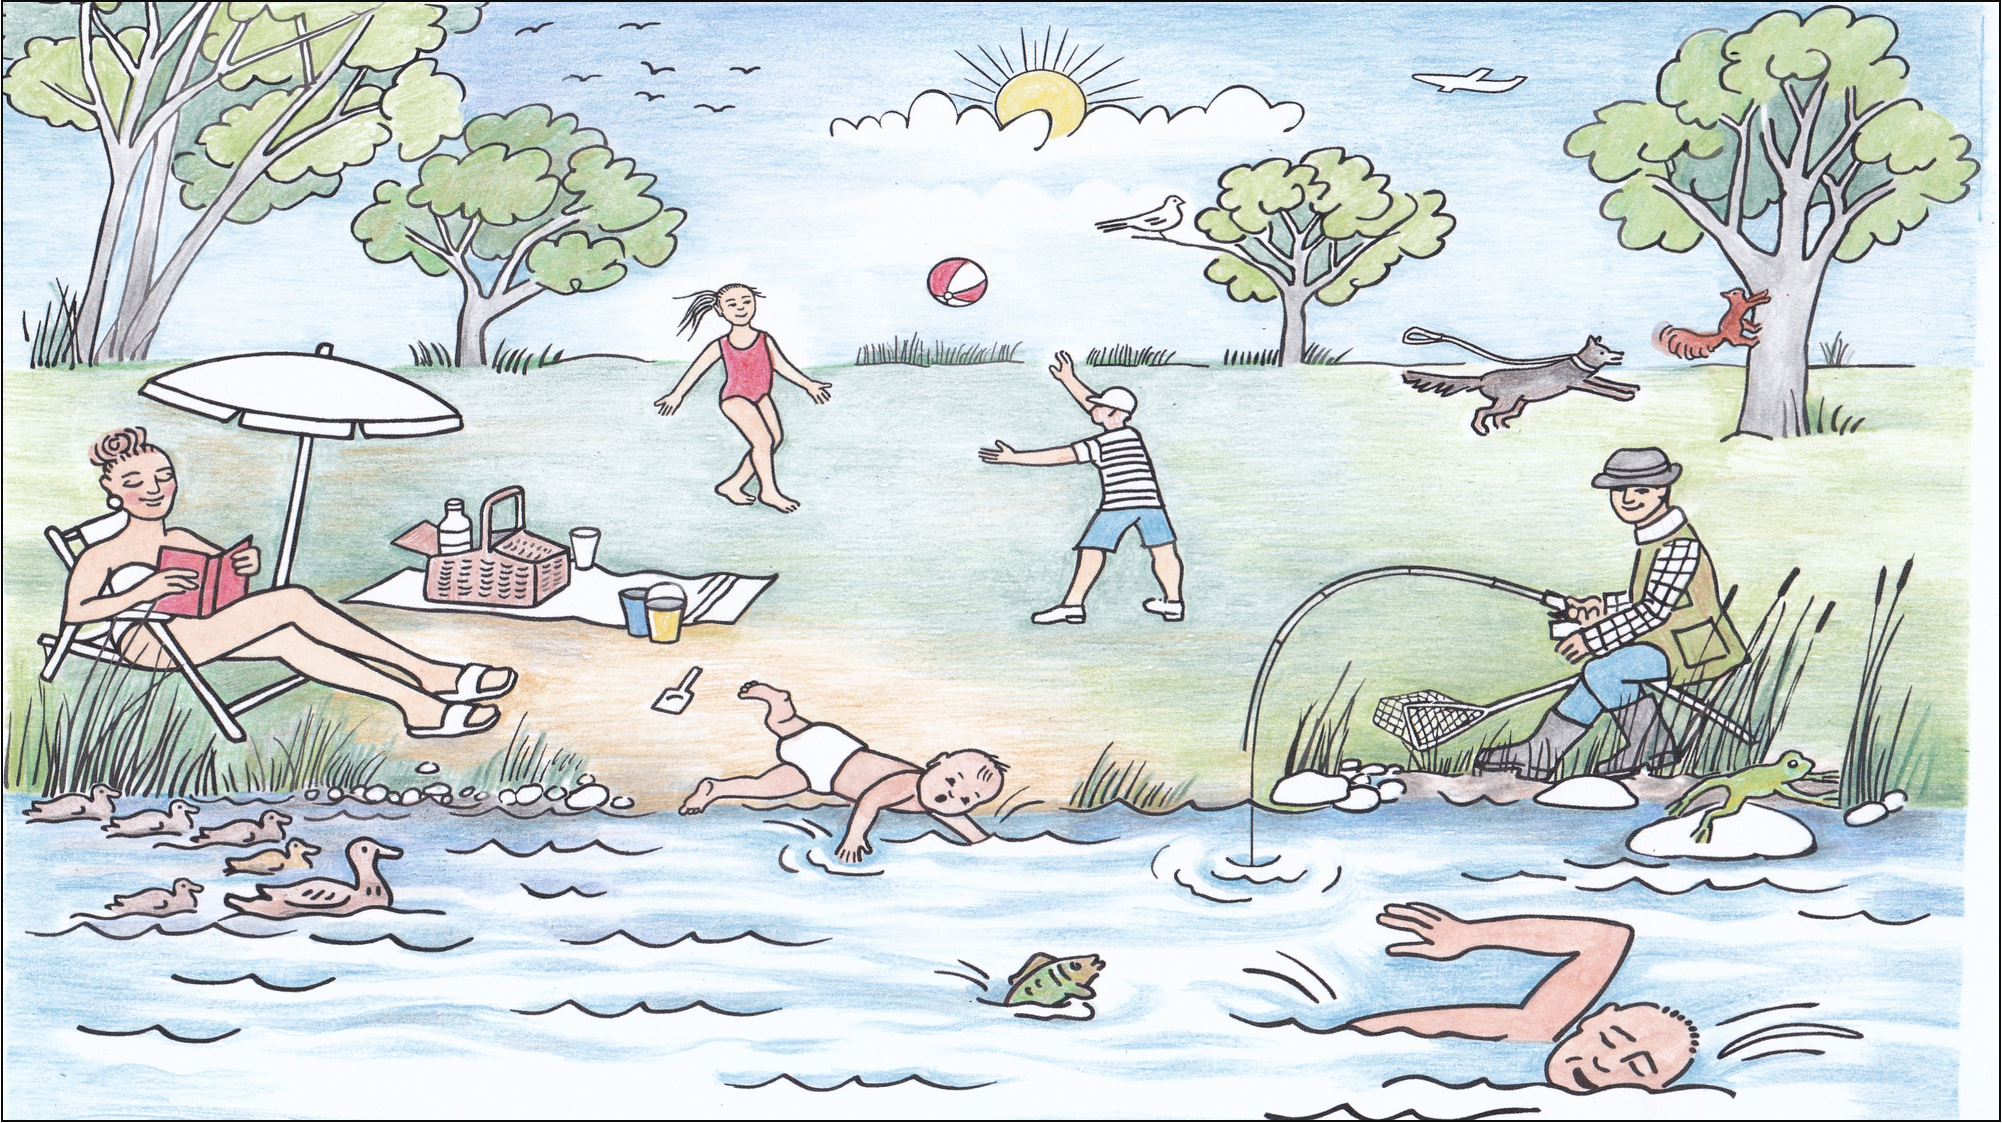
\includegraphics[width=\textwidth]{./src/imgs/summer.png}
	\caption{Kresba použitá pro testování}\label{fig:summer}
\end{figure}

Jak bylo definováno v kapitole~\ref{subsec:reprezentace_znalosti}, referenční popis obrázku se skládá z
množiny objektů, jejich atributů a vazeb mezi nimi.
Nyní bylo potřeba stanovit nějaký datový formát, který by umožnil tuto strukturu dobře zachytit.

\newpage
Základním prvkem referenčního popisu je struktura \enquote{\texttt{Scene}}, která obsahuje informace o obrázku, objekty s atributy a vazby mezi nimi.

Objekty byly definované strukturou \enquote{\texttt{SceneObject}}, která popisuje objekt ve scéně a jeho atributy.
Každý \texttt{SceneObject} obsahuje informaci o svém názvu, umístění, velikosti a hierarchii vůči ostatním objektům.
Dále si každý \texttt{SceneObject} udržuje list atributů a tagů, které mu byly expertem přiděleny.

Další strukturou, která byla definována jako součást referenčního popisu, je \enquote{\texttt{Triplet}}.
Tato struktura slouží k popisu vazeb mezi objekty, obsahuje názvy dvou objektů a k nim název vazby.

Schéma implementovaných struktur a jejich provázání je na Obrázku~\ref{fig:schema_impl_ref_popis}.
Zkratka pro datový typ \texttt{u32} znamená \enquote{unsigned 32-bit int} a je to nezáporné celé číslo na 32 bitech,
druhý typ \texttt{Vec<T>} pak značí vektor (list) objektů typu \texttt{T}.

\begin{figure}[ht!]
	\centering
	\begin{tikzpicture}
		\node[inner sep=0] (ref) at (0, 0) {
			\begin{tabular}{|l|l|l|}
				\hline
				\multicolumn{2}{|c|}{\large \texttt{Scene}}                    \\
				\hline
				\textbf{\textit{Pole}} & \textbf{\textit{Datový typ}}          \\
				\hline
				{width}                & \texttt{u32}                          \\
				{height}               & \texttt{u32}                          \\
				{image\_path}          & \texttt{String}                       \\
				{objects}              & \texttt{Vec<\phantom{ SceneObject }>} \\
				{triplets}             & \texttt{Vec<\phantom{ Triplet }>}     \\
				\hline
			\end{tabular}
		};
		\node[anchor=north, inner sep=1pt] (trip) at ($(ref.south) + (0, -1)$) {
			\begin{tabular}{|l|l|l|}
				\hline
				\multicolumn{2}{|c|}{\large \texttt{Triplet}}         \\
				\hline
				\textbf{\textit{Pole}} & \textbf{\textit{Datový typ}} \\
				\hline
				{from}                 & \texttt{String}              \\
				{predicate}            & \texttt{String}              \\
				{to}                   & \texttt{String}              \\
				\hline
			\end{tabular}
		};
		\node[anchor=north west, inner sep=1pt] (so) at ($(trip.north east) + (1, 0)$) {
			\begin{tabular}{|l|l|l|}
				\hline
				\multicolumn{2}{|c|}{\large \texttt{SceneObject}}       \\
				\hline
				\textbf{\textit{Pole}} & \textbf{\textit{Datový typ}}   \\
				\hline
				{name}                 & \texttt{String}                \\
				{tags}                 & \texttt{Vec<String>}           \\
				{top\_left\_corner}    & \texttt{(u32, u32)}            \\
				{size}                 & \texttt{(u32, u32)}            \\
				{parents}              & \texttt{Vec<String>}           \\
				{children}             & \texttt{Vec<String>}           \\
				{attributes}           & \texttt{Vec<(String, String)>} \\
				\hline
			\end{tabular}
		};
		\node[anchor=south east] (somark) at ($(ref.south east) + (-14.5pt, \baselineskip)$) {\texttt{SceneObject}};
		\node[anchor=south east] (trmark) at ($(ref.south east) + (-39.5pt, 0)$) {\texttt{Triplet}};
		\node[draw=blue, thick,rounded corners=2mm, inner sep=3pt] (trborder) at ($(trmark) + (0, 0.5pt)$) {{\phantom{\texttt{Triplet}}}};
		\node[draw=blue,thick, rounded corners=2mm, inner sep=3pt] (soborder) at ($(somark) + (0, 0.5pt)$) {{\phantom{\texttt{SceneObject}}}};
		\draw[blue,thick, -Stealth] (trborder.south) to (trmark|-trip.north);
		\draw[blue,thick, rounded corners=2mm, -Stealth] (soborder.north) -- ++(0, 0.5) -| (so.north);
		% \draw[blue, rounded corners=3mm, -Stealth] (soborder.north) |- ($(0, 0.2) + (so.west)$);
	\end{tikzpicture}
	\caption{Schéma implementace referenčního popisu}\label{fig:schema_impl_ref_popis}
\end{figure}

Ve struktuře \texttt{Scene} je význam jednotlivých polí poměrně jednoduchý.
Pole \texttt{width} a \texttt{height} vyjadřují výšku a šířku obrázku v pixelech, \texttt{image\_path} udává cestu k souboru, který obsahuje samotný obrázek.
Pole \texttt{objects} a \texttt{triplets} pak obsahují list objektů a tripletů.

Struktura \texttt{Triplet} je velmi jednoduchá.
Její pole \texttt{from} a \texttt{to} jsou názvy zdrojového, respektive cílového, objektu.
Pole \texttt{predicate} je název samotné vazby mezi těmito objekty.

Poslední struktura \texttt{SceneObject}, která popisuje samotné objekty, je nejsložitější.
Pole \texttt{name} udává název daného objektu, který slouží zároveň jako identifikátor a musí být tudíž unikátní.
Může nastat situace, že v obrázku bude více objektů, které by přirozeně byly označené stejně, například dva stromy.
Pro tento případ byla implementována možnost objekty číslovat a tím tak jednoznačně rozlišit i objekty stejného typu.
Číslování objektů je součástí jejich názvu a má formát \enquote{\texttt{\#n}} kde $n$ je přirozené číslo označující index objektu.
Například \enquote{\texttt{strom \#1}} a \enquote{\texttt{strom \#2}}.

Dvojice polí \texttt{top\_left\_corner} a \texttt{size} udávají velikost a pozici objektu zdrojovém obrázku.
Jedná se o souřadnice levého horního rohu ohraničujícího rámce (bounding-boxu) a velikost tohoto rámce v pixelech.
Obě pole mají jako uvedený datový typ \texttt{(u32, u32)}, který reprezentuje souřadnice $(i, j)$ kde $i,j \in \mathbb{N}^{0}$.
V obrázku je jako počátek souřadnic uvažován levý horní roh.

Pole \texttt{tags} reprezentuje list tagů, které expert obrázku přiřadil.
Jejich účel byl popsán v kapitole~\ref{subsec:hodnoceni}.
Další dvojice polí \texttt{parents} a \texttt{children} pak reprezentuje list objektů, které jsou rodiče, respektive potomci, daného objektu.

Po formální definice formátů a datový typů bylo potřeba určit, jakým způsobem bude expert referenční popis tvořit.
Pro tuto práci bylo rozhodnuto, že tvorba referenčního popisu bude spočívat v napsání strukturovaného textového souboru.
Zvolen byl textový formát \texttt{JSON}, který představuje dobrý kompromis mezi čitelností člověkem a strojovou zpracovatelností.

Ukázka části referenčního popisu je na Výpisu~\ref{lst:ref_popis_real_example}.
\clearpage
% \def\lstlabel{label=}
\begin{lstlisting}[
	% there are many more options of styling, see the official documentation, these are just the defaults I like
	frame=single, % make single-line frame around the verbatim
	framesep=2mm, % put some more spacing between the frame and text
	aboveskip=5mm, % put some more space above the box
	basicstyle={\linespread{0.83}\footnotesize\ttfamily}, % use typewriter (monospace) font
	caption={Příklad jednoduchého referenčního popisu}, % set the caption text
	captionpos=b, % put the caption at the bottom (b) or top (t) or both (bt)
	label={lst:ref_popis_real_example}, % label to be referenced via \ref{}
	numbers=left, % line numbers on the left
	numberstyle={\scriptsize\ttfamily\color{black!60}}, % the style for line numbers
	escapeinside={<@}{@>} % between those sequences are command evaluated
]
<@\textcolor[HTML]{FF1010}{\texttt{\{}}@>
<@\textcolor[HTML]{000000}{\texttt{\ \ }}@><@\textcolor[HTML]{255CFF}{\texttt{"width"}}@><@\textcolor[HTML]{1041FF}{\texttt{:}}@><@\textcolor[HTML]{000000}{\texttt{\ }}@><@\textcolor[HTML]{DE6F10}{\texttt{2002}}@><@\textcolor[HTML]{1041FF}{\texttt{,}}@>
<@\textcolor[HTML]{000000}{\texttt{\ \ }}@><@\textcolor[HTML]{255CFF}{\texttt{"height"}}@><@\textcolor[HTML]{1041FF}{\texttt{:}}@><@\textcolor[HTML]{000000}{\texttt{\ }}@><@\textcolor[HTML]{DE6F10}{\texttt{1123}}@><@\textcolor[HTML]{1041FF}{\texttt{,}}@>
<@\textcolor[HTML]{000000}{\texttt{\ \ }}@><@\textcolor[HTML]{255CFF}{\texttt{"image\_path"}}@><@\textcolor[HTML]{1041FF}{\texttt{:}}@><@\textcolor[HTML]{000000}{\texttt{\ }}@><@\textcolor[HTML]{418310}{\texttt{"./data/imgs/summer.png"}}@><@\textcolor[HTML]{1041FF}{\texttt{,}}@>
<@\textcolor[HTML]{000000}{\texttt{\ \ }}@><@\textcolor[HTML]{255CFF}{\texttt{"objects"}}@><@\textcolor[HTML]{1041FF}{\texttt{:}}@><@\textcolor[HTML]{000000}{\texttt{\ }}@><@\textcolor[HTML]{FF1010}{\texttt{[}}@>
<@\textcolor[HTML]{000000}{\texttt{\ \ \ \ }}@><@\textcolor[HTML]{FF1010}{\texttt{\{}}@>
<@\textcolor[HTML]{000000}{\texttt{\ \ \ \ \ \ }}@><@\textcolor[HTML]{255CFF}{\texttt{"name"}}@><@\textcolor[HTML]{1041FF}{\texttt{:}}@><@\textcolor[HTML]{000000}{\texttt{\ }}@><@\textcolor[HTML]{418310}{\texttt{"tree\ \#1"}}@><@\textcolor[HTML]{1041FF}{\texttt{,}}@>
<@\textcolor[HTML]{000000}{\texttt{\ \ \ \ \ \ }}@><@\textcolor[HTML]{255CFF}{\texttt{"tags"}}@><@\textcolor[HTML]{1041FF}{\texttt{:}}@><@\textcolor[HTML]{000000}{\texttt{\ }}@><@\textcolor[HTML]{FF1010}{\texttt{[}}@><@\textcolor[HTML]{418310}{\texttt{"environment"}}@><@\textcolor[HTML]{FF1010}{\texttt{]}}@><@\textcolor[HTML]{1041FF}{\texttt{,}}@>
<@\textcolor[HTML]{000000}{\texttt{\ \ \ \ \ \ }}@><@\textcolor[HTML]{255CFF}{\texttt{"top\_left\_corner"}}@><@\textcolor[HTML]{1041FF}{\texttt{:}}@><@\textcolor[HTML]{000000}{\texttt{\ }}@><@\textcolor[HTML]{FF1010}{\texttt{[}}@><@\textcolor[HTML]{DE6F10}{\texttt{1194}}@><@\textcolor[HTML]{1041FF}{\texttt{,}}@><@\textcolor[HTML]{000000}{\texttt{\ }}@><@\textcolor[HTML]{DE6F10}{\texttt{146}}@><@\textcolor[HTML]{FF1010}{\texttt{]}}@><@\textcolor[HTML]{1041FF}{\texttt{,}}@>
<@\textcolor[HTML]{000000}{\texttt{\ \ \ \ \ \ }}@><@\textcolor[HTML]{255CFF}{\texttt{"size"}}@><@\textcolor[HTML]{1041FF}{\texttt{:}}@><@\textcolor[HTML]{000000}{\texttt{\ }}@><@\textcolor[HTML]{FF1010}{\texttt{[}}@><@\textcolor[HTML]{DE6F10}{\texttt{264}}@><@\textcolor[HTML]{1041FF}{\texttt{,}}@><@\textcolor[HTML]{000000}{\texttt{\ }}@><@\textcolor[HTML]{DE6F10}{\texttt{220}}@><@\textcolor[HTML]{FF1010}{\texttt{]}}@><@\textcolor[HTML]{1041FF}{\texttt{,}}@>
<@\textcolor[HTML]{000000}{\texttt{\ \ \ \ \ \ }}@><@\textcolor[HTML]{255CFF}{\texttt{"parents"}}@><@\textcolor[HTML]{1041FF}{\texttt{:}}@><@\textcolor[HTML]{000000}{\texttt{\ }}@><@\textcolor[HTML]{FF1010}{\texttt{[}}@><@\textcolor[HTML]{FF1010}{\texttt{]}}@><@\textcolor[HTML]{1041FF}{\texttt{,}}@>
<@\textcolor[HTML]{000000}{\texttt{\ \ \ \ \ \ }}@><@\textcolor[HTML]{255CFF}{\texttt{"children"}}@><@\textcolor[HTML]{1041FF}{\texttt{:}}@><@\textcolor[HTML]{000000}{\texttt{\ }}@><@\textcolor[HTML]{FF1010}{\texttt{[}}@><@\textcolor[HTML]{418310}{\texttt{"branch"}}@><@\textcolor[HTML]{FF1010}{\texttt{]}}@><@\textcolor[HTML]{1041FF}{\texttt{,}}@>
<@\textcolor[HTML]{000000}{\texttt{\ \ \ \ \ \ }}@><@\textcolor[HTML]{255CFF}{\texttt{"attributes"}}@><@\textcolor[HTML]{1041FF}{\texttt{:}}@><@\textcolor[HTML]{000000}{\texttt{\ }}@><@\textcolor[HTML]{FF1010}{\texttt{[}}@>
<@\textcolor[HTML]{000000}{\texttt{\ \ \ \ \ \ \ \ }}@><@\textcolor[HTML]{FF1010}{\texttt{[}}@><@\textcolor[HTML]{418310}{\texttt{"color"}}@><@\textcolor[HTML]{1041FF}{\texttt{,}}@><@\textcolor[HTML]{000000}{\texttt{\ }}@><@\textcolor[HTML]{418310}{\texttt{"green"}}@><@\textcolor[HTML]{FF1010}{\texttt{]}}@><@\textcolor[HTML]{1041FF}{\texttt{,}}@>
<@\textcolor[HTML]{000000}{\texttt{\ \ \ \ \ \ \ \ }}@><@\textcolor[HTML]{FF1010}{\texttt{[}}@><@\textcolor[HTML]{418310}{\texttt{"color"}}@><@\textcolor[HTML]{1041FF}{\texttt{,}}@><@\textcolor[HTML]{000000}{\texttt{\ }}@><@\textcolor[HTML]{418310}{\texttt{"brown"}}@><@\textcolor[HTML]{FF1010}{\texttt{]}}@>
<@\textcolor[HTML]{000000}{\texttt{\ \ \ \ \ \ }}@><@\textcolor[HTML]{FF1010}{\texttt{]}}@>
<@\textcolor[HTML]{000000}{\texttt{\ \ \ \ }}@><@\textcolor[HTML]{FF1010}{\texttt{\}}}@><@\textcolor[HTML]{1041FF}{\texttt{,}}@> <@\textcolor[HTML]{FF1010}{\texttt{\{}}@>
<@\textcolor[HTML]{000000}{\texttt{\ \ \ \ \ \ }}@><@\textcolor[HTML]{255CFF}{\texttt{"name"}}@><@\textcolor[HTML]{1041FF}{\texttt{:}}@><@\textcolor[HTML]{000000}{\texttt{\ }}@><@\textcolor[HTML]{418310}{\texttt{"bird"}}@><@\textcolor[HTML]{1041FF}{\texttt{,}}@>
<@\textcolor[HTML]{000000}{\texttt{\ \ \ \ \ \ }}@><@\textcolor[HTML]{255CFF}{\texttt{"tags"}}@><@\textcolor[HTML]{1041FF}{\texttt{:}}@><@\textcolor[HTML]{000000}{\texttt{\ }}@><@\textcolor[HTML]{FF1010}{\texttt{[}}@><@\textcolor[HTML]{418310}{\texttt{"animal"}}@><@\textcolor[HTML]{FF1010}{\texttt{]}}@><@\textcolor[HTML]{1041FF}{\texttt{,}}@>
<@\textcolor[HTML]{000000}{\texttt{\ \ \ \ \ \ }}@><@\textcolor[HTML]{255CFF}{\texttt{"top\_left\_corner"}}@><@\textcolor[HTML]{1041FF}{\texttt{:}}@><@\textcolor[HTML]{000000}{\texttt{\ }}@><@\textcolor[HTML]{FF1010}{\texttt{[}}@><@\textcolor[HTML]{DE6F10}{\texttt{1095}}@><@\textcolor[HTML]{1041FF}{\texttt{,}}@><@\textcolor[HTML]{000000}{\texttt{\ }}@><@\textcolor[HTML]{DE6F10}{\texttt{193}}@><@\textcolor[HTML]{FF1010}{\texttt{]}}@><@\textcolor[HTML]{1041FF}{\texttt{,}}@>
<@\textcolor[HTML]{000000}{\texttt{\ \ \ \ \ \ }}@><@\textcolor[HTML]{255CFF}{\texttt{"size"}}@><@\textcolor[HTML]{1041FF}{\texttt{:}}@><@\textcolor[HTML]{000000}{\texttt{\ }}@><@\textcolor[HTML]{FF1010}{\texttt{[}}@><@\textcolor[HTML]{DE6F10}{\texttt{93}}@><@\textcolor[HTML]{1041FF}{\texttt{,}}@><@\textcolor[HTML]{000000}{\texttt{\ }}@><@\textcolor[HTML]{DE6F10}{\texttt{47}}@><@\textcolor[HTML]{FF1010}{\texttt{]}}@><@\textcolor[HTML]{1041FF}{\texttt{,}}@>
<@\textcolor[HTML]{000000}{\texttt{\ \ \ \ \ \ }}@><@\textcolor[HTML]{255CFF}{\texttt{"parents"}}@><@\textcolor[HTML]{1041FF}{\texttt{:}}@><@\textcolor[HTML]{000000}{\texttt{\ }}@><@\textcolor[HTML]{FF1010}{\texttt{[}}@><@\textcolor[HTML]{FF1010}{\texttt{]}}@><@\textcolor[HTML]{1041FF}{\texttt{,}}@>
<@\textcolor[HTML]{000000}{\texttt{\ \ \ \ \ \ }}@><@\textcolor[HTML]{255CFF}{\texttt{"children"}}@><@\textcolor[HTML]{1041FF}{\texttt{:}}@><@\textcolor[HTML]{000000}{\texttt{\ }}@><@\textcolor[HTML]{FF1010}{\texttt{[}}@><@\textcolor[HTML]{FF1010}{\texttt{]}}@><@\textcolor[HTML]{1041FF}{\texttt{,}}@>
<@\textcolor[HTML]{000000}{\texttt{\ \ \ \ \ \ }}@><@\textcolor[HTML]{255CFF}{\texttt{"attributes"}}@><@\textcolor[HTML]{1041FF}{\texttt{:}}@><@\textcolor[HTML]{000000}{\texttt{\ }}@><@\textcolor[HTML]{FF1010}{\texttt{[}}@><@\textcolor[HTML]{FF1010}{\texttt{[}}@><@\textcolor[HTML]{418310}{\texttt{"color"}}@><@\textcolor[HTML]{1041FF}{\texttt{,}}@><@\textcolor[HTML]{000000}{\texttt{\ }}@><@\textcolor[HTML]{418310}{\texttt{"white"}}@><@\textcolor[HTML]{FF1010}{\texttt{]}}@><@\textcolor[HTML]{FF1010}{\texttt{]}}@>
<@\textcolor[HTML]{000000}{\texttt{\ \ \ \ }}@><@\textcolor[HTML]{FF1010}{\texttt{\}}}@><@\textcolor[HTML]{1041FF}{\texttt{,}}@> <@\textcolor[HTML]{FF1010}{\texttt{\{}}@>
<@\textcolor[HTML]{000000}{\texttt{\ \ \ \ \ \ }}@><@\textcolor[HTML]{255CFF}{\texttt{"name"}}@><@\textcolor[HTML]{1041FF}{\texttt{:}}@><@\textcolor[HTML]{000000}{\texttt{\ }}@><@\textcolor[HTML]{418310}{\texttt{"squirrel"}}@><@\textcolor[HTML]{1041FF}{\texttt{,}}@>
<@\textcolor[HTML]{000000}{\texttt{\ \ \ \ \ \ }}@><@\textcolor[HTML]{255CFF}{\texttt{"tags"}}@><@\textcolor[HTML]{1041FF}{\texttt{:}}@><@\textcolor[HTML]{000000}{\texttt{\ }}@><@\textcolor[HTML]{FF1010}{\texttt{[}}@><@\textcolor[HTML]{418310}{\texttt{"animal"}}@><@\textcolor[HTML]{FF1010}{\texttt{]}}@><@\textcolor[HTML]{1041FF}{\texttt{,}}@>
<@\textcolor[HTML]{000000}{\texttt{\ \ \ \ \ \ }}@><@\textcolor[HTML]{255CFF}{\texttt{"top\_left\_corner"}}@><@\textcolor[HTML]{1041FF}{\texttt{:}}@><@\textcolor[HTML]{000000}{\texttt{\ }}@><@\textcolor[HTML]{FF1010}{\texttt{[}}@><@\textcolor[HTML]{DE6F10}{\texttt{1655}}@><@\textcolor[HTML]{1041FF}{\texttt{,}}@><@\textcolor[HTML]{000000}{\texttt{\ }}@><@\textcolor[HTML]{DE6F10}{\texttt{286}}@><@\textcolor[HTML]{FF1010}{\texttt{]}}@><@\textcolor[HTML]{1041FF}{\texttt{,}}@>
<@\textcolor[HTML]{000000}{\texttt{\ \ \ \ \ \ }}@><@\textcolor[HTML]{255CFF}{\texttt{"size"}}@><@\textcolor[HTML]{1041FF}{\texttt{:}}@><@\textcolor[HTML]{000000}{\texttt{\ }}@><@\textcolor[HTML]{FF1010}{\texttt{[}}@><@\textcolor[HTML]{DE6F10}{\texttt{116}}@><@\textcolor[HTML]{1041FF}{\texttt{,}}@><@\textcolor[HTML]{000000}{\texttt{\ }}@><@\textcolor[HTML]{DE6F10}{\texttt{76}}@><@\textcolor[HTML]{FF1010}{\texttt{]}}@><@\textcolor[HTML]{1041FF}{\texttt{,}}@>
<@\textcolor[HTML]{000000}{\texttt{\ \ \ \ \ \ }}@><@\textcolor[HTML]{255CFF}{\texttt{"parents"}}@><@\textcolor[HTML]{1041FF}{\texttt{:}}@><@\textcolor[HTML]{000000}{\texttt{\ }}@><@\textcolor[HTML]{FF1010}{\texttt{[}}@><@\textcolor[HTML]{FF1010}{\texttt{]}}@><@\textcolor[HTML]{1041FF}{\texttt{,}}@>
<@\textcolor[HTML]{000000}{\texttt{\ \ \ \ \ \ }}@><@\textcolor[HTML]{255CFF}{\texttt{"children"}}@><@\textcolor[HTML]{1041FF}{\texttt{:}}@><@\textcolor[HTML]{000000}{\texttt{\ }}@><@\textcolor[HTML]{FF1010}{\texttt{[}}@><@\textcolor[HTML]{FF1010}{\texttt{]}}@><@\textcolor[HTML]{1041FF}{\texttt{,}}@>
<@\textcolor[HTML]{000000}{\texttt{\ \ \ \ \ \ }}@><@\textcolor[HTML]{255CFF}{\texttt{"attributes"}}@><@\textcolor[HTML]{1041FF}{\texttt{:}}@><@\textcolor[HTML]{000000}{\texttt{\ }}@><@\textcolor[HTML]{FF1010}{\texttt{[}}@>
<@\textcolor[HTML]{000000}{\texttt{\ \ \ \ \ \ \ \ }}@><@\textcolor[HTML]{FF1010}{\texttt{[}}@><@\textcolor[HTML]{418310}{\texttt{"color"}}@><@\textcolor[HTML]{1041FF}{\texttt{,}}@><@\textcolor[HTML]{000000}{\texttt{\ }}@><@\textcolor[HTML]{418310}{\texttt{"orange"}}@><@\textcolor[HTML]{FF1010}{\texttt{]}}@><@\textcolor[HTML]{1041FF}{\texttt{,}}@>
<@\textcolor[HTML]{000000}{\texttt{\ \ \ \ \ \ \ \ }}@><@\textcolor[HTML]{FF1010}{\texttt{[}}@><@\textcolor[HTML]{418310}{\texttt{"color"}}@><@\textcolor[HTML]{1041FF}{\texttt{,}}@><@\textcolor[HTML]{000000}{\texttt{\ }}@><@\textcolor[HTML]{418310}{\texttt{"brown"}}@><@\textcolor[HTML]{FF1010}{\texttt{]}}@>
<@\textcolor[HTML]{000000}{\texttt{\ \ \ \ \ \ }}@><@\textcolor[HTML]{FF1010}{\texttt{]}}@>
<@\textcolor[HTML]{000000}{\texttt{\ \ \ \ }}@><@\textcolor[HTML]{FF1010}{\texttt{\}}}@><@\textcolor[HTML]{1041FF}{\texttt{,}}@> <@\textcolor[HTML]{FF1010}{\texttt{\{}}@>
<@\textcolor[HTML]{000000}{\texttt{\ \ \ \ \ \ }}@><@\textcolor[HTML]{255CFF}{\texttt{"name"}}@><@\textcolor[HTML]{1041FF}{\texttt{:}}@><@\textcolor[HTML]{000000}{\texttt{\ }}@><@\textcolor[HTML]{418310}{\texttt{"bird"}}@><@\textcolor[HTML]{1041FF}{\texttt{,}}@>
<@\textcolor[HTML]{000000}{\texttt{\ \ \ \ \ \ }}@><@\textcolor[HTML]{255CFF}{\texttt{"tags"}}@><@\textcolor[HTML]{1041FF}{\texttt{:}}@><@\textcolor[HTML]{000000}{\texttt{\ }}@><@\textcolor[HTML]{FF1010}{\texttt{[}}@><@\textcolor[HTML]{418310}{\texttt{"animal"}}@><@\textcolor[HTML]{FF1010}{\texttt{]}}@><@\textcolor[HTML]{1041FF}{\texttt{,}}@>
<@\textcolor[HTML]{000000}{\texttt{\ \ \ \ \ \ }}@><@\textcolor[HTML]{255CFF}{\texttt{"top\_left\_corner"}}@><@\textcolor[HTML]{1041FF}{\texttt{:}}@><@\textcolor[HTML]{000000}{\texttt{\ }}@><@\textcolor[HTML]{FF1010}{\texttt{[}}@><@\textcolor[HTML]{DE6F10}{\texttt{1095}}@><@\textcolor[HTML]{1041FF}{\texttt{,}}@><@\textcolor[HTML]{000000}{\texttt{\ }}@><@\textcolor[HTML]{DE6F10}{\texttt{193}}@><@\textcolor[HTML]{FF1010}{\texttt{]}}@><@\textcolor[HTML]{1041FF}{\texttt{,}}@>
<@\textcolor[HTML]{000000}{\texttt{\ \ \ \ \ \ }}@><@\textcolor[HTML]{255CFF}{\texttt{"size"}}@><@\textcolor[HTML]{1041FF}{\texttt{:}}@><@\textcolor[HTML]{000000}{\texttt{\ }}@><@\textcolor[HTML]{FF1010}{\texttt{[}}@><@\textcolor[HTML]{DE6F10}{\texttt{93}}@><@\textcolor[HTML]{1041FF}{\texttt{,}}@><@\textcolor[HTML]{000000}{\texttt{\ }}@><@\textcolor[HTML]{DE6F10}{\texttt{47}}@><@\textcolor[HTML]{FF1010}{\texttt{]}}@><@\textcolor[HTML]{1041FF}{\texttt{,}}@>
<@\textcolor[HTML]{000000}{\texttt{\ \ \ \ \ \ }}@><@\textcolor[HTML]{255CFF}{\texttt{"parents"}}@><@\textcolor[HTML]{1041FF}{\texttt{:}}@><@\textcolor[HTML]{000000}{\texttt{\ }}@><@\textcolor[HTML]{FF1010}{\texttt{[}}@><@\textcolor[HTML]{FF1010}{\texttt{]}}@><@\textcolor[HTML]{1041FF}{\texttt{,}}@>
<@\textcolor[HTML]{000000}{\texttt{\ \ \ \ \ \ }}@><@\textcolor[HTML]{255CFF}{\texttt{"children"}}@><@\textcolor[HTML]{1041FF}{\texttt{:}}@><@\textcolor[HTML]{000000}{\texttt{\ }}@><@\textcolor[HTML]{FF1010}{\texttt{[}}@><@\textcolor[HTML]{FF1010}{\texttt{]}}@><@\textcolor[HTML]{1041FF}{\texttt{,}}@>
<@\textcolor[HTML]{000000}{\texttt{\ \ \ \ \ \ }}@><@\textcolor[HTML]{255CFF}{\texttt{"attributes"}}@><@\textcolor[HTML]{1041FF}{\texttt{:}}@><@\textcolor[HTML]{000000}{\texttt{\ }}@><@\textcolor[HTML]{FF1010}{\texttt{[}}@><@\textcolor[HTML]{FF1010}{\texttt{[}}@><@\textcolor[HTML]{418310}{\texttt{"color"}}@><@\textcolor[HTML]{1041FF}{\texttt{,}}@><@\textcolor[HTML]{000000}{\texttt{\ }}@><@\textcolor[HTML]{418310}{\texttt{"white"}}@><@\textcolor[HTML]{FF1010}{\texttt{]}}@><@\textcolor[HTML]{FF1010}{\texttt{]}}@>
<@\textcolor[HTML]{000000}{\texttt{\ \ \ \ }}@><@\textcolor[HTML]{FF1010}{\texttt{\}}}@><@\textcolor[HTML]{1041FF}{\texttt{,}}@> <@\textcolor[HTML]{FF1010}{\texttt{\{}}@>
<@\textcolor[HTML]{000000}{\texttt{\ \ \ \ \ \ }}@><@\textcolor[HTML]{255CFF}{\texttt{"name"}}@><@\textcolor[HTML]{1041FF}{\texttt{:}}@><@\textcolor[HTML]{000000}{\texttt{\ }}@><@\textcolor[HTML]{418310}{\texttt{"branch"}}@><@\textcolor[HTML]{1041FF}{\texttt{,}}@>
<@\textcolor[HTML]{000000}{\texttt{\ \ \ \ \ \ }}@><@\textcolor[HTML]{255CFF}{\texttt{"tags"}}@><@\textcolor[HTML]{1041FF}{\texttt{:}}@><@\textcolor[HTML]{000000}{\texttt{\ }}@><@\textcolor[HTML]{FF1010}{\texttt{[}}@><@\textcolor[HTML]{418310}{\texttt{"environment"}}@><@\textcolor[HTML]{1041FF}{\texttt{,}}@><@\textcolor[HTML]{000000}{\texttt{\ }}@><@\textcolor[HTML]{418310}{\texttt{"background"}}@><@\textcolor[HTML]{FF1010}{\texttt{]}}@><@\textcolor[HTML]{1041FF}{\texttt{,}}@>
<@\textcolor[HTML]{000000}{\texttt{\ \ \ \ \ \ }}@><@\textcolor[HTML]{255CFF}{\texttt{"top\_left\_corner"}}@><@\textcolor[HTML]{1041FF}{\texttt{:}}@><@\textcolor[HTML]{000000}{\texttt{\ }}@><@\textcolor[HTML]{FF1010}{\texttt{[}}@><@\textcolor[HTML]{DE6F10}{\texttt{1130}}@><@\textcolor[HTML]{1041FF}{\texttt{,}}@><@\textcolor[HTML]{000000}{\texttt{\ }}@><@\textcolor[HTML]{DE6F10}{\texttt{233}}@><@\textcolor[HTML]{FF1010}{\texttt{]}}@><@\textcolor[HTML]{1041FF}{\texttt{,}}@>
<@\textcolor[HTML]{000000}{\texttt{\ \ \ \ \ \ }}@><@\textcolor[HTML]{255CFF}{\texttt{"size"}}@><@\textcolor[HTML]{1041FF}{\texttt{:}}@><@\textcolor[HTML]{000000}{\texttt{\ }}@><@\textcolor[HTML]{FF1010}{\texttt{[}}@><@\textcolor[HTML]{DE6F10}{\texttt{138}}@><@\textcolor[HTML]{1041FF}{\texttt{,}}@><@\textcolor[HTML]{000000}{\texttt{\ }}@><@\textcolor[HTML]{DE6F10}{\texttt{41}}@><@\textcolor[HTML]{FF1010}{\texttt{]}}@><@\textcolor[HTML]{1041FF}{\texttt{,}}@>
<@\textcolor[HTML]{000000}{\texttt{\ \ \ \ \ \ }}@><@\textcolor[HTML]{255CFF}{\texttt{"parents"}}@><@\textcolor[HTML]{1041FF}{\texttt{:}}@><@\textcolor[HTML]{000000}{\texttt{\ }}@><@\textcolor[HTML]{FF1010}{\texttt{[}}@><@\textcolor[HTML]{418310}{\texttt{"tree\ \#1"}}@><@\textcolor[HTML]{FF1010}{\texttt{]}}@><@\textcolor[HTML]{1041FF}{\texttt{,}}@>
<@\textcolor[HTML]{000000}{\texttt{\ \ \ \ \ \ }}@><@\textcolor[HTML]{255CFF}{\texttt{"children"}}@><@\textcolor[HTML]{1041FF}{\texttt{:}}@><@\textcolor[HTML]{000000}{\texttt{\ }}@><@\textcolor[HTML]{FF1010}{\texttt{[}}@><@\textcolor[HTML]{FF1010}{\texttt{]}}@><@\textcolor[HTML]{1041FF}{\texttt{,}}@>
<@\textcolor[HTML]{000000}{\texttt{\ \ \ \ \ \ }}@><@\textcolor[HTML]{255CFF}{\texttt{"attributes"}}@><@\textcolor[HTML]{1041FF}{\texttt{:}}@><@\textcolor[HTML]{000000}{\texttt{\ }}@><@\textcolor[HTML]{FF1010}{\texttt{[}}@><@\textcolor[HTML]{FF1010}{\texttt{]}}@>
<@\textcolor[HTML]{000000}{\texttt{\ \ \ \ }}@><@\textcolor[HTML]{FF1010}{\texttt{\}}}@>
<@\textcolor[HTML]{000000}{\texttt{\ \ }}@><@\textcolor[HTML]{FF1010}{\texttt{]}}@><@\textcolor[HTML]{1041FF}{\texttt{,}}@>
<@\textcolor[HTML]{000000}{\texttt{\ \ }}@><@\textcolor[HTML]{255CFF}{\texttt{"triplets"}}@><@\textcolor[HTML]{1041FF}{\texttt{:}}@><@\textcolor[HTML]{000000}{\texttt{\ }}@><@\textcolor[HTML]{FF1010}{\texttt{[}}@>
<@\textcolor[HTML]{000000}{\texttt{\ \ \ \ }}@><@\textcolor[HTML]{FF1010}{\texttt{\{}}@><@\textcolor[HTML]{255CFF}{\texttt{"from"}}@><@\textcolor[HTML]{1041FF}{\texttt{:}}@><@\textcolor[HTML]{000000}{\texttt{\ }}@><@\textcolor[HTML]{418310}{\texttt{"bird"}}@><@\textcolor[HTML]{1041FF}{\texttt{,}}@><@\textcolor[HTML]{000000}{\texttt{\ }}@><@\textcolor[HTML]{255CFF}{\texttt{"predicate"}}@><@\textcolor[HTML]{1041FF}{\texttt{:}}@><@\textcolor[HTML]{000000}{\texttt{\ }}@><@\textcolor[HTML]{418310}{\texttt{"sitting\ on"}}@><@\textcolor[HTML]{1041FF}{\texttt{,}}@><@\textcolor[HTML]{000000}{\texttt{\ }}@><@\textcolor[HTML]{255CFF}{\texttt{"to"}}@><@\textcolor[HTML]{1041FF}{\texttt{:}}@><@\textcolor[HTML]{000000}{\texttt{\ }}@><@\textcolor[HTML]{418310}{\texttt{"branch"}}@><@\textcolor[HTML]{FF1010}{\texttt{\}}}@><@\textcolor[HTML]{1041FF}{\texttt{,}}@>
<@\textcolor[HTML]{000000}{\texttt{\ \ \ \ }}@><@\textcolor[HTML]{FF1010}{\texttt{\{}}@><@\textcolor[HTML]{255CFF}{\texttt{"from"}}@><@\textcolor[HTML]{1041FF}{\texttt{:}}@><@\textcolor[HTML]{000000}{\texttt{\ }}@><@\textcolor[HTML]{418310}{\texttt{"bird"}}@><@\textcolor[HTML]{1041FF}{\texttt{,}}@><@\textcolor[HTML]{000000}{\texttt{\ }}@><@\textcolor[HTML]{255CFF}{\texttt{"predicate"}}@><@\textcolor[HTML]{1041FF}{\texttt{:}}@><@\textcolor[HTML]{000000}{\texttt{\ }}@><@\textcolor[HTML]{418310}{\texttt{"sitting\ on"}}@><@\textcolor[HTML]{1041FF}{\texttt{,}}@><@\textcolor[HTML]{000000}{\texttt{\ }}@><@\textcolor[HTML]{255CFF}{\texttt{"to"}}@><@\textcolor[HTML]{1041FF}{\texttt{:}}@><@\textcolor[HTML]{000000}{\texttt{\ }}@><@\textcolor[HTML]{418310}{\texttt{"tree\ \#1"}}@><@\textcolor[HTML]{FF1010}{\texttt{\}}}@><@\textcolor[HTML]{1041FF}{\texttt{,}}@>
<@\textcolor[HTML]{000000}{\texttt{\ \ \ \ }}@><@\textcolor[HTML]{FF1010}{\texttt{\{}}@><@\textcolor[HTML]{255CFF}{\texttt{"from"}}@><@\textcolor[HTML]{1041FF}{\texttt{:}}@><@\textcolor[HTML]{000000}{\texttt{\ }}@><@\textcolor[HTML]{418310}{\texttt{"squirrel"}}@><@\textcolor[HTML]{1041FF}{\texttt{,}}@><@\textcolor[HTML]{000000}{\texttt{\ }}@><@\textcolor[HTML]{255CFF}{\texttt{"predicate"}}@><@\textcolor[HTML]{1041FF}{\texttt{:}}@><@\textcolor[HTML]{000000}{\texttt{\ }}@><@\textcolor[HTML]{418310}{\texttt{"climbing"}}@><@\textcolor[HTML]{1041FF}{\texttt{,}}@><@\textcolor[HTML]{000000}{\texttt{\ }}@><@\textcolor[HTML]{255CFF}{\texttt{"to"}}@><@\textcolor[HTML]{1041FF}{\texttt{:}}@><@\textcolor[HTML]{000000}{\texttt{\ }}@><@\textcolor[HTML]{418310}{\texttt{"tree\ \#1"}}@><@\textcolor[HTML]{FF1010}{\texttt{\}}}@><@\textcolor[HTML]{1041FF}{\texttt{,}}@>
<@\textcolor[HTML]{000000}{\texttt{\ \ \ \ }}@><@\textcolor[HTML]{FF1010}{\texttt{\{}}@><@\textcolor[HTML]{255CFF}{\texttt{"from"}}@><@\textcolor[HTML]{1041FF}{\texttt{:}}@><@\textcolor[HTML]{000000}{\texttt{\ }}@><@\textcolor[HTML]{418310}{\texttt{"squirrel"}}@><@\textcolor[HTML]{1041FF}{\texttt{,}}@><@\textcolor[HTML]{000000}{\texttt{\ }}@><@\textcolor[HTML]{255CFF}{\texttt{"predicate"}}@><@\textcolor[HTML]{1041FF}{\texttt{:}}@><@\textcolor[HTML]{000000}{\texttt{\ }}@><@\textcolor[HTML]{418310}{\texttt{"under"}}@><@\textcolor[HTML]{1041FF}{\texttt{,}}@><@\textcolor[HTML]{000000}{\texttt{\ }}@><@\textcolor[HTML]{255CFF}{\texttt{"to"}}@><@\textcolor[HTML]{1041FF}{\texttt{:}}@><@\textcolor[HTML]{000000}{\texttt{\ }}@><@\textcolor[HTML]{418310}{\texttt{"bird"}}@><@\textcolor[HTML]{FF1010}{\texttt{\}}}@>
<@\textcolor[HTML]{000000}{\texttt{\ \ }}@><@\textcolor[HTML]{FF1010}{\texttt{]}}@>
<@\textcolor[HTML]{FF1010}{\texttt{\}}}@>

\end{lstlisting}


\subsubsection{Validace referenčního popisu}
Jak bylo právě ukázáno, tvorba referenčního popisu je ve své podstatě psaní JSON souboru podle nějaké definované struktury a pravidel.
Program při zpracovávání referenčního popisu předpokládá, že data budou validní a odmítne referenční popis, který by obsahoval chyby.
Pro komplexnější scénu však může být náročné pro lidského experta neudělat v popise žádnou chybu a udržet celý referenční popis validní.

Z toho důvodu byl implementován v rámci celého programu příkaz \texttt{check}, který zajišťuje kontrolu všech dříve definovaných pravidel, které musí referenční popis splňovat:
\begin{enumerate}
	\item \textbf{Kontrola názvů objektů}\\
	      Protože je název objektu použit jako identifikátor, tak musí být unikátní a žádné dva objekty ve scéně nesmí mít shodný název.
	      V případě, že by referenční popis obsahoval duplicitní názvy objektů, program na tyto konflikty upozorní.
	\item \textbf{Kontrola přetékání objektů}\\
	      Jelikož má program k dispozici informace o velikosti obrázku (v pixelech) a zároveň pro jednotlivé objekty také jejich pozici a velikost,
	      tak lze předem ověřit, zda uvedené ohraničující rámce nezasahují mimo obrázek.
	      Pokud se tak stane, program vypíše varovné hlášení a upozorní na jednotlivé problematické hodnoty.
	\item \textbf{Kontrola referencí na objekty}\\
	      Objekty mohou v rámci hierarchie odkazovat na jiné objekty.
	      Aby byly tyto reference validní, tak objekt nesmí odkazovat sám na sebe, referovaný objekt musí existovat a hierarchické vazby musí být oboustranné.
	      Tím je myšleno to, že pokud objekt \texttt{\color{red!80!black}A} specifikuje objekt \texttt{\color{red!80!black}B} jako svého rodiče,
	      pak musí i objekt \texttt{\color{red!80!black}B} specifikovat \texttt{\color{red!80!black}A} jako svého potomka a naopak.

	      V případě, že by byly detekované nějaké invalidní odkazy, bude opět vypsáno varovné hlášení o tom, co je v referenčním popise špatně.
	\item \textbf{Kontrola referencí v tripletech}\\
	      Při specifikaci vazeb mezi objekty jsou také odkazované dva objekty.
	      Aby byl triplet validní, musí být oba referované objekty definované ve scéně.
	      V opačném případě bude vypsáno chybové hlášení s informací o chybějících objekty v tripletech.
\end{enumerate}

\subsubsection{Další příkazy pro práci s referenčním popisem}
Kromě příkazu na kontrolu referenčního popisu byly implementované ještě následující pomocné příkazy.
Tyto příkazy slouží obecně k prohlížení a porovnávání referenčních popisů a byly implementované zejména pro situace, kdy by bylo potřeba analyzovat komplexnější scény, porovnávat je mezi sebou a získat obecný přehled o scéně, aniž by potřeba zkoumat samotné JSON soubory.
\begin{enumerate}
	\item \textbf{Příkaz} \texttt{stats}: \\
	      Tento příkaz vypíše základní vybrané statistiky daného referenčního popisu.
	      Hlavním smyslem tohoto příkazu je poskytnout člověku představu o referenčním popisu k němu příslušejícímu obrázku.

	      Příkaz vypíše cestu k souboru s referenčním popisem, dále cestu k souboru,
	      který obsahuje popisovaný obrázek a jeho velikost v pixelech.
	      Dále vypíše počet objektů a počet vazeb (tripletů), které byly v tomto referenčním popise definované.
	\item \textbf{Příkaz} \texttt{list}: \\
	      Příkaz \texttt{list} slouží k vypsání seznamu všech entit daného typu, podobně jako při použití databázových dotazů.
	      Tento příkaz má několik pod-příkazů, které určují, jaký typ informace má být vypsán v podobě seznamu.
	      Může se jednat o objekty, tagy, triplety, atributy, samotné názvy nebo hodnoty atributů,
	      názvy vazeb mezi objekty a další.
	      Seznam všech implementovaných pod-příkazů je možné si prohlédnout ve zdrojovém kódu.

	      Cílem tohoto příkazu je poskytnout rychlý a pohodlný způsob, jak získat seznam všech prvků daného typu ve scéně, aniž by bylo potřeba přímo pracovat se složitější strukturou JSON souboru.
	      Výstup je formátován tak, aby jej bylo možné snadno dále strojově zpracovat a integrovat do komplexnějších sekvencí příkazů.
	\item \textbf{Příkaz} \texttt{crumble}: \\
	      Referenční popis obrazu byl v této práci definován jako množina objektů, jejich atributů a vazeb mezi objekty.
	      Při pohledu na datový typ atributu a tripletu je ale možné si všimnout, že se v podstatě neliší - obojí se skládá ze tří částí,
	      jejichž obsah může být zaměnitelný a rozdíl ve významu je dán pouze zavedenou interpretací.
	      Bylo by tedy možné zobecnit všechny tyto entity a popsat je pouze jedním atomickým datovým typem, který obsahuje dva prvky a vazbu mezi nimi.
	      V této podobě by bylo možné celý referenční popis zobrazit jako tradiční sémantickou síť, kde není rozlišeno, co je vazba mezi objekty a co je pouze popis vlastnosti.

	      Referenční popis nebyl navržen tímto obecnějším způsobem z toho důvodu, že pro komplexnější scény by počet těchto atomických trojic dosahoval tak vysokých hodnot,
	      že by pro lidského experta bylo velmi obtížné se v datech orientovat.
	      Pro strojové zpracování a případné vizualizace by ale mohlo být prospěšné, aby byly všechny typy informací prezentované v jednoduchém formátu.
	      Právě k tomu slouží příkaz \texttt{crumble}, který, jak již název napovídá, daný referenční popis \enquote{rozdrobí} a převede všechny informace do množiny prostých trojic.

	      Schématická ukázka procesu \enquote{rozdrobení} je na Obrázku~\ref{fig:crumble_example}.
	      % malý kluk v modrém tričku chytá červený míč
	      \begin{figure}[ht!]
		      \centering
		      \begin{tikzpicture}
			      \footnotesize
			      \matrix[draw, anchor=west] (boy) at (0, 0) {
				      \node {{\textbf{kluk}}}; \\
				      \node {\texttt{stáří:}}; &
				      \node {\texttt{\textit{mladý}}};                 \\
				      \node {\texttt{výraz:}}; &
				      \node {\texttt{\textit{úsměv}}};                 \\
			      };
			      \matrix[draw, anchor=west] (tshirt) at (1.75, -3) {
				      \node  {{\textbf{tričko}}}; \\
				      \node {\texttt{barva:}}; &
				      \node {\texttt{\textit{zelená}}};                  \\
			      };
			      \matrix[draw, anchor=west] (ball) at (-1.75, -3) {
				      \node  {{\textbf{míč}}}; \\
				      \node {\texttt{barva:}}; &
				      \node {\texttt{\textit{červená}}};                  \\
			      };
			      \draw[-Stealth] (boy) to node[midway, above, sloped] {chytá} (ball);
			      \draw[-Stealth] (boy) to node[midway, above, sloped] {nosí} (tshirt);
			      \matrix[draw, anchor=west] (crumb) at ($0.5*(boy.north) + 0.25*(ball.south) + 0.25*(tshirt.south) + (4, 0)$) {
				      \node {\texttt{kluk - stáří - mladý}}; \\
				      \node {\texttt{kluk - výraz - úsměv}}; \\
				      \node {\texttt{kluk - chytá - míč}}; \\
				      \node {\texttt{kluk - nosí - tričko}}; \\
				      \node {\texttt{míč - barva - červená}}; \\
				      \node {\texttt{tričko - barva - zelená}}; \\
			      };
			      \draw[-Stealth] ($(crumb.west) + (-1.5, 0)$) to node[midway, above] {\texttt{crumble}} ($(crumb.west) + (-0.2, 0)$);
		      \end{tikzpicture}
		      \caption{Ukázka procesu \texttt{crumble} (\enquote{rozdrobení})}\label{fig:crumble_example}
	      \end{figure}

	\item \textbf{Příkaz} \texttt{render}: \\
	      Tento příkaz slouží k vytvoření vizuální reprezentace referenčního popisu.

	      Pro správnou funkci tohoto příkazu je nutné, aby byl na počítači dostupný program Graphviz~\cite{graphviz},
	      jehož DOT-engine je použitý pro vytvoření grafické reprezentace.
	      Výhodou grafické prezentace je přehlednost pro člověka, nicméně pro velmi komplexní scény s mnoha vazbami ani grafická reprezentace nemusí být dostatečná.
	      Je vhodné zmínit, že jedním z problémů takto implementované vizualizace je to, že pro scény s mnoha objekty tvoří Graphviz velmi dlouhé a úzké obrázky,
	      protože sázecí mechanismus skládá jednotlivé uzly pod sebe.

	      Grafická prezentace a metody vizualizace jsou nad rámec zadání této práce, proto bylo rozhodnuto, že pro ilustraci tato implementace dostačuje a případné komplexnější
	      způsoby grafické prezentace jsou ponechány jako možná budoucí rozšíření.
\end{enumerate}


\subsection{Sémantické parsování pomocí gramatik}\label{subsec:moje_gramatiky}
Extrakce sémantické informace byla jednou z hlavních řešených problematik.
Jak již bylo řečeno dříve, byl zvolen přístup založený na parsování textu pomocí sémantických bezkontextových gramatik.

Při prvotních experimentech byla použita již existující implementace tohoto konceptu,
\todo{referovat na SpeechCloud}
používající standard SRGS~\cite{srgs}.

Během těchto prvních pokusů ale bylo zjištěno, že funkcionalita, kterou nabízí existující implementace,
nebude pro potřeby této práce postačovat.
Kvůli tomu byla navržena, implementována a otestována vlastní realizace stejného konceptu
analýzy textu pomocí bezkontextových gramatik, která lépe vyhovovala ostatním zde navrženým,
realizovaným a popsaným postupům a metodám.

Detaily této vlastní implementace a rozdíly oproti existujícím variantám jsou popsány v následujících kapitolách.

\subsubsection{Problémy s existující implementací a SRGS}
Při práci s existující implementací SRGS standardu (SpeechCloud)
\todo{referovat SC správně formálně}
vyvstaly následující problémy:
\begin{enumerate}
	\item \textbf{Speciální pravidlo \texttt{\$GARBAGE}}\\
	      První problém, který bylo potřeba vyřešit, byla absence pravidla \texttt{\$GARBAGE}.
	      Jedná se o speciální pravidlo definované ve standardu SRGS, které má tu vlastnost, že dokáže reprezentovat libovolnou promluvu nebo libovolný token.

	      Lze tak velmi efektivně využít v situacích, kdy je potřeba specifikovat výplňová slova,
	      která dopředu není možné odhadnout a nebo nás při analýze textu nezajímají.

	      Existující implementace však neměla toto speciální pravidlo implementováno.
	      To představovalo problém, protože možnost specifikovat libovolný token je jeden ze základních konceptů,
	      na kterém byl celý navržený koncept sémantické analýzy postaven.
	\item \textbf{Návratová datová struktura}\\
	      Existující implementace nevracela ze svého API celý derivační strom, ale pouze list tagů, které se v derivačním stromu nacházely.
	      To znamená, že byla ztracena hierarchická informace derivačního stromu spolu s informací o konkrétních pravidlech,
	      které byly během zpracování textu použité.

	      Tyto informace nebyly zcela nezbytné pro další postup, avšak jejich absence by
	      vyžadovala výrazně složitější definici parsovacích pravidel v bezkontextových gramatikách a
	      s tím samozřejmě spojený složitější systém na zpracování obdržených výsledků.

	      Dostupnost celých derivačních stromů by tedy byla výhodná ve smyslu zjednodušení dalšího postupu.
	\item \textbf{Řešení nejednoznačných situací}\\
	      Třetí problém vycházel z toho, že SRGS standard umožňuje existenci některých situací,
	      kde není jednoznačně dáno, jak má parsování probíhat,
	      a teoreticky je možné získat z jednoho vstupu více různých derivačních stromů.


	      Existující implementace tyto situace dokázala zpracovat, avšak vrátila pouze jeden výsledek,
	      který byl považovaný za nejlepší podle daného kritéria - v tomto případě podle délky zpracovaného textu.

	      Pro sémantickou analýzu textu potřebnou pro získání testovaného popisu by ale bylo výhodné,
	      kdyby bylo možné toto kritérium změnit, a nebo ještě lépe, získat všechna možná řešení.
\end{enumerate}

Po důkladném zvážení těchto problémů bylo rozhodnuto,
že jako nejlepší způsob řešení bude implementace vlastního parseru.

Během reimplementace vlastního parseru byla jako základní reference využita specifikace SRGS~\cite{srgs},
která přesně popisuje chování, funkčnost i syntax gramatik.

V průběhu reimplementace byly ovšem za účelem zjednodušení vynechány některé části SRGS standardu,
které by pro sémantickou analýzu textu v této práci nebyly nijak užitečné a naopak byly přidány nějaké funkce navíc,
které byly pak využity ve zbytku práce.

Výsledkem tak byl nový formát, označený \enquote{Semantic Parsing Grammar Format} (SPGF).
K němu byly samozřejmě vytvořené i základní softwarové nástroje, které nabízí:
\begin{itemize}
	\item kontrolu syntaxe a případné hlášení o syntaktických chybách,
	\item TreeSitter~\cite{treesitter} modul pro obarvení SPGF kódu v textových editorech,
	\item parser SPGF syntaxe s validací obsahu gramatiky i jednotlivých pravidel,
	\item parser přirozeného textu, který využívá právě SPGF gramatiky.
\end{itemize}

\subsubsection{Semantic Parsing Grammar Format (SPGF)}\label{subsubsec:spgf_def}
Základním a nejvyšším prvkem SPGF je \emph{gramatika}.
Na rozdíl od SRGS definice, SPGF gramatika nevyžaduje žádnou hlavičku a nepodporuje dodatečné prvky,
jako deklaraci jazyka nebo meta-dat.
Gramatika má podobu textového souboru, ve kterém je definována množina parsovacích pravidel.

Každé pravidlo se skládá ze svého názvu, který je uvozený symbolem \enquote{\texttt{\$}}.
Název pravidla slouží jako identifikátor, musí být tedy unikátní v dané gramatice.
Druhou částí pravidla je expanze, která reprezentuje tělo pravidla.
Mezi názvem a expanzí pravidla je znak rovnítka \enquote{=}.
Pravidlo je vždy zakončeno středníkem.
Například:
\begin{center}
	\begin{tikzpicture}
		\node[inner sep=0] (dolar) at (0, 0) {\texttt{\strut\$}};
		\node[inner sep=0,anchor=west] (name) at (dolar.east) {\texttt{\strut climbing}};
		\node[inner sep=0,anchor=west] (eq) at (name.east) {\texttt{\strut\phantom{a}=\phantom{a}}};
		\node[inner sep=0,anchor=west] (body) at (eq.east) {\texttt{\strut (leze | šplhá) [na | po]}};
		\node[inner sep=0,anchor=west] (sc) at (body.east) {\texttt{\strut;}};

		\def\downdist{0.0}
		\draw[thick, decorate, decoration={calligraphic brace, mirror, amplitude=4}]
		($(name.south west) + (0, \downdist)$) -- ($(name.south east) + (0, \downdist)$)
		node[pos=0.5, below=3pt] {\scriptsize název pravidla};
		\draw[thick, decorate, decoration={calligraphic brace, mirror, amplitude=4}]
		($(body.south west) + (0, \downdist)$) -- ($(body.south east) + (0, \downdist)$)
		node[pos=0.5, below=3pt] {\scriptsize expanze (tělo pravidla)};
	\end{tikzpicture}
\end{center}

Tělo pravidla se skládá z takzvaných \emph{alternativ}, které jsou oddělené znakem \enquote{\texttt{|}}.
Tato \emph{alternativa} je pak dále definována jako posloupnost \emph{elementů}.
V zápise má přednost mezera před \enquote{\texttt{|}}, takže několik tokenů po sobě je bráno jako jeden celek.
Element má tři varianty, může jím být \emph{token, reference} nebo \emph{sekvence}.
Například:

\begin{center}
	\begin{tikzpicture}
		\node[inner sep=0] (name) at (0, 0) {\texttt{\strut\$dog =\phantom{a}}};
		\node[inner sep=0,anchor=west] (pejsek) at (name.east) {\texttt{\strut pejsek}};
		\node[inner sep=0,anchor=west] (s) at (pejsek.east) {\texttt{\strut\phantom{a}}};
		\node[inner sep=0,anchor=west] (p) at (s.east) {\texttt{\strut |}};
		\node[inner sep=0,anchor=west] (s) at (p.east) {\texttt{\strut\phantom{a}}};
		\node[inner sep=0,anchor=west] (b1) at (s.east) {\texttt{\strut (}};
		\node[inner sep=0,anchor=west] (pes) at (b1.east) {\texttt{\strut pes}};
		\node[inner sep=0,anchor=west] (s) at (pes.east) {\texttt{\strut\phantom{a}}};
		\node[inner sep=0,anchor=west] (p) at (s.east) {\texttt{\strut |}};
		\node[inner sep=0,anchor=west] (s) at (p.east) {\texttt{\strut\phantom{a}}};
		\node[inner sep=0,anchor=west] (psík) at (s.east) {\texttt{\strut psík}};
		\node[inner sep=0,anchor=west] (b2) at (psík.east) {\texttt{\strut )}};
		\node[inner sep=0,anchor=west] (s) at (b2.east) {\texttt{\strut\phantom{a}}};
		\node[inner sep=0,anchor=west] (p) at (s.east) {\texttt{\strut |}};
		\node[inner sep=0,anchor=west] (s) at (p.east) {\texttt{\strut\phantom{a}}};
		\node[inner sep=0,anchor=west] (nej) at (s.east) {\texttt{\strut nejlepší}};
		\node[inner sep=0,anchor=west] (s) at (nej.east) {\texttt{\strut\phantom{a}}};
		\node[inner sep=0,anchor=west] (friend) at (s.east) {\texttt{\strut přítel}};
		\node[inner sep=0,anchor=west] (s) at (friend.east) {\texttt{\strut\phantom{a}}};
		\node[inner sep=0,anchor=west] (human) at (s.east) {\texttt{\strut člověka}};
		\node[inner sep=0,anchor=west] (semicolon) at (human.east) {\texttt{\strut ;}};

		\def\downdist{0.0}
		\draw[thick, decorate, decoration={calligraphic brace, mirror, amplitude=4}]
		($(pejsek.south west) + (0, \downdist)$) -- ($(pejsek.south east) + (0, \downdist)$)
		node[pos=0.5, above=-16pt] {\scriptsize alternativa 1};
		\draw[thick, decorate, decoration={calligraphic brace, mirror, amplitude=4}]
		($(b1.south west) + (0, \downdist)$) -- ($(b2.south east) + (0, \downdist)$)
		node[pos=0.5, above=-16pt] {\scriptsize alternativa 2};
		\draw[thick, decorate, decoration={calligraphic brace, mirror, amplitude=4}]
		($(nej.south west) + (0, \downdist)$) -- ($(human.south east) + (0, \downdist)$)
		node[pos=0.5, above=-16pt] {\scriptsize alternativa 3};

		\def\updist{0.1}

		\draw[thick, decorate, decoration={calligraphic brace, amplitude=4}]
		($(pejsek.north west) + (0, -\updist)$) -- ($(pejsek.north east) + (0, -\updist)$)
		node[pos=0.5, above=3pt] {\scriptsize token};

		% \draw[thick, decorate, decoration={calligraphic brace, amplitude=4}]
		% ($(pes.north west) + (0, -\updist)$) -- ($(pes.north east) + (0, -\updist)$)
		% node[pos=0.5, above=3pt] {\scriptsize token};

		% \draw[thick, decorate, decoration={calligraphic brace, amplitude=4}]
		% ($(psík.north west) + (0, -\updist)$) -- ($(psík.north east) + (0, -\updist)$)
		% node[pos=0.5, above=3pt] {\scriptsize token};

		\draw[thick, decorate, decoration={calligraphic brace, amplitude=4}]
		($(nej.north west) + (0, -\updist)$) -- ($(nej.north east) + (0, -\updist)$)
		node[pos=0.5, above=3pt] {\scriptsize token};

		\draw[thick, decorate, decoration={calligraphic brace, amplitude=4}]
		($(friend.north west) + (0, -\updist)$) -- ($(friend.north east) + (0, -\updist)$)
		node[pos=0.5, above=3pt] {\scriptsize token};

		\draw[thick, decorate, decoration={calligraphic brace, amplitude=4}]
		($(human.north west) + (0, -\updist)$) -- ($(human.north east) + (0, -\updist)$)
		node[pos=0.5, above=3pt] {\scriptsize token};

		\draw[thick, decorate, decoration={calligraphic brace, amplitude=4}]
		($(b1.north west) + (0, -\updist)$) -- ($(b2.north east) + (0, -\updist)$)
		node[pos=0.5, above=3pt] {\scriptsize sekvence};
	\end{tikzpicture}
\end{center}

Nejjednodušší variantou \emph{elementu} je \emph{token}.
Jedná se o terminální symbol (literál), který udává, jaký řetězec je při parsování právě přípustný.
Token je možné chápat jako konkrétní slovo, které je v dané pozici v textu očekávané.
Může se skládat z jednoho nebo více znaků, která mohou být písmena, číslice, tečka, pomlčka, podtržítko nebo dvojtečka.
Součástí definice tokenu může také být (volitelně) definice opakování a případně libovolný počet tagů.
Opakování elementů a tagy budou detailněji popsány později.

Druhou variantou elementu je \emph{reference}.
Tímto pojmem se rozumí odkaz na jiné pravidlo, a nebo odkaz na nějaké speciální pravidlo s vyhrazeným názvem.
Reference začíná symbolem \enquote{\texttt{\$}} po kterém následuje okamžitě (bez mezery) jméno referovaného
pravidla definovaného ve stejné gramatice, nebo speciálního pravidla.
SPGF umožňuje referovat pravidla rekurzivně, a to jak přímo (pravidlo obsahuje referenci na samo sebe), tak v cyklu.

Například jednoduchá gramatika pro (fiktivní) zápis vybraných matematických operací obsahuje rekurzivní pravidlo \texttt{\$expr}:
\begin{verbatim}
	public $expr = $numer | $expr $operator $expr;
	public $number = $digit<+>;
	public $digit = 0 | 1 | 2 | 3 | 4 | 5 | 6 | 7 | 8 | 9 | 10;
	public $operator = plus | minus | dot | frac ;
\end{verbatim}

Formát SPGF definuje 5 speciálních pravidel s vyhraněnými jmény.
Tři z nich jsou převzaté ze SRGS standardu, zbylé dvě byly přidány navíc, aby bylo možné vynutit jistá chování parsovacího algoritmu,
která jsou v SRGS automaticky, ale v SPGF nikoli, kvůli odlišné strategii prohledávání (viz později).
\begin{enumerate}
	\item \textbf{Speciální pravidlo} \texttt{\$GARBAGE}:\\
	      Akceptuje libovolný jeden token a posune parsování o akceptovaný token dále.

	      Speciální pravidlo \texttt{\$GARBAGE} je užitečné, když je potřeba vyjádřit, že na dané pozici v textu
	      může být libovolné slovo, které buďto nedokážeme předvídat, nebo nás nezajímá.
	\item \textbf{Speciální pravidlo} \texttt{\$NULL}:\\
	      Akceptuje prázdný řetězec.
	      To znamená, že je vždy úspěšně aktivováno a nikdy neposune parsování o žádný znak dále.

	      Lze využít například pro situace, kde je žádoucí přidat do derivačního stromu (angl.~parsing tree) nějaké tagy,
	      aniž by byl učiněn postup v parsovaném textu.
	\item \textbf{Speciální pravidlo} \texttt{\$VOID}:\\
	      Vždy selže, bez ohledu na parsovaný text.
	      Nikdy tedy není úspěšné a sekvence obsahující \texttt{\$VOID} také nikdy nebude úspěšná.

	      Lze využít například pro dočasné blokování některých jiných pravidel, nebo pro zdůraznění,
	      že daná sekvence tokenů se nesmí v textu vyskytovat.
	\item \textbf{Speciální pravidlo} \texttt{\$END}:\\
	      Akceptuje konec textu.
	      Bude úspěšné právě ve chvíli, kdy je parsování na konci textu a nezbývá již žádný znak ke zpracování.

	      Umístění speciálního pravidla \texttt{\$END} na konec nějaké expanze tak způsobí,
	      že celá expanze bude úspěšná pouze ve chvíli, kdy dokáže pojmout text beze zbytku až do konce.
	\item \textbf{Speciální pravidlo} \texttt{\$BEGIN}: \\
	      Akceptuje začátek textu.
	      Bude úspěšné právě ve chvíli, kdy je parsování na začátku textu a žádný znak ještě nebyl zpracován.

	      Umístění speciálního pravidla \texttt{\$BEGIN} na začátek expanze tak způsobí,
	      že celá expanze bude úspěšná pouze ve chvíli, kdy dokáže pojmout text od prvního znaku.
\end{enumerate}

Poslední podobu, kterou \emph{element} může mít, je \emph{sekvence}.
Sekvence může být \enquote{obyčejná} nebo \enquote{volitelná}.
V~obou případech se jedná o \emph{alternativy} oddělené znakem \enquote{\texttt{|}},
list alternativ je ohraničený kulatými, respektive hranatými, závorkami.

Důvodem pro existenci \emph{sekvencí} je to, že umožňují seskupování elementů a přehlednější tvorbu složitějších konstrukcí,
podobně jako jsou v matematice používané závorky v aritmetických či algebraických výrazech.
Volitelná sekvence (s hranatými závorkami) je pouze syntaktická zkratka pro \enquote{obyčejnou} sekvenci,
která má minimální počet opakování roven nule (takže se nemusí vůbec v textu vyskytovat) a
maximální počet opakování roven jedné.
Jedná se o obdobu operátoru \enquote{\texttt{?}} v regulárních výrazech.

Příklad zápisu pravidla s oběma typy sekvencí a jeho schématická reprezentace
je pak na Obrázku~\ref{fig:climbing_rule_scheme}.
\begin{figure}[H]
	\centering
	\begin{tikzpicture}
		\node[inner sep=0] (dolar) at (0, 0) {\texttt{\strut\$}};
		\node[inner sep=0,anchor=west] (name) at (dolar.east) {\texttt{\strut climbing}};
		\node[inner sep=0,anchor=west] (eq) at (name.east) {\texttt{\strut\phantom{a}=\phantom{a}}};
		\node[inner sep=0,anchor=west] (b1) at (eq.east) {\texttt{\strut (}};
		\node[inner sep=0,anchor=west] (s) at (b1.east) {\texttt{\strut\phantom{a}}};
		\node[inner sep=0,anchor=west] (leze) at (s.east) {\texttt{\strut leze}};
		\node[inner sep=0,anchor=west] (s) at (leze.east) {\texttt{\strut\phantom{a}}};
		\node[inner sep=0,anchor=west] (p) at (s.east) {\texttt{\strut |}};
		\node[inner sep=0,anchor=west] (s) at (p.east) {\texttt{\strut\phantom{a}}};
		\node[inner sep=0,anchor=west] (šplhá) at (s.east) {\texttt{\strut šplhá}};
		\node[inner sep=0,anchor=west] (s) at (šplhá.east) {\texttt{\strut\phantom{a}}};
		\node[inner sep=0,anchor=west] (b2) at (s.east) {\texttt{\strut )}};
		\node[inner sep=0,anchor=west] (s) at (b2.east) {\texttt{\strut\phantom{a}}};
		\node[inner sep=0,anchor=west] (b3) at (s.east) {\texttt{\strut [}};
		\node[inner sep=0,anchor=west] (s) at (b3.east) {\texttt{\strut\phantom{a}}};
		\node[inner sep=0,anchor=west] (na) at (s.east) {\texttt{\strut na}};
		\node[inner sep=0,anchor=west] (s) at (na.east) {\texttt{\strut\phantom{a}}};
		\node[inner sep=0,anchor=west] (p) at (s.east) {\texttt{\strut |}};
		\node[inner sep=0,anchor=west] (s) at (p.east) {\texttt{\strut\phantom{a}}};
		\node[inner sep=0,anchor=west] (po) at (s.east) {\texttt{\strut po}};
		\node[inner sep=0,anchor=west] (s) at (po.east) {\texttt{\strut\phantom{a}}};
		\node[inner sep=0,anchor=west] (b4) at (s.east) {\texttt{\strut ]}};
		\node[inner sep=0,anchor=west] (sem) at (b4.east) {\texttt{\strut;}};

		\def\downdist{0.0}
		\draw[thick, decorate, decoration={calligraphic brace, mirror, amplitude=4}]
		($(b1.south west) + (0, \downdist)$) -- ($(b2.south east) + (0, \downdist)$)
		node[pos=0.5, below=3pt] {\scriptsize sekvence};

		\draw[thick, decorate, decoration={calligraphic brace, mirror, amplitude=4}]
		($(b3.south west) + (0, \downdist)$) -- ($(b4.south east) + (0, \downdist)$)
		node[pos=0.5, below=3pt] {\scriptsize volitelná sekvence};

		\def\downdist{-0.1}
		\draw[thick, decorate, decoration={calligraphic brace, amplitude=4}]
		($(leze.north west) + (0, \downdist)$) -- ($(šplhá.north east) + (0, \downdist)$)
		node[pos=0.5, above=3pt] {\scriptsize 2 alternativy};
		\draw[thick, decorate, decoration={calligraphic brace, amplitude=4}]
		($(na.north west) + (0, \downdist)$) -- ($(po.north east) + (0, \downdist)$)
		node[pos=0.5, above=3pt] {\scriptsize 2 alternativy};
	\end{tikzpicture}

	\phantom{a} % spacing between the pictures

	\begin{tikzpicture}[inner sep=0pt,rounded corners=2mm]
		\node[draw, minimum width=17mm] (leze) at (0, 0.6) {\texttt{\strut leze}};
		\node[draw, minimum width=17mm] (šplhá) at (0, -0.6)  {\texttt{\strut šplhá}};
		\node[circle,fill,minimum width=5pt] (begin) at ($(leze.west) + (-1, -0.6)$) {};
		\node[draw, minimum width=10mm] (na) at ($(leze) + (3, 0.0)$)  {\texttt{\strut na}};
		\node[draw, minimum width=10mm] (po) at ($(šplhá) + (3, -0.0)$)  {\texttt{\strut po}};
		\node[circle,fill,minimum width=5pt] (end) at ($(na.east) + (1.2, -0.6)$) {};

		\draw[-Stealth] (begin.center) -- ++(0.5, 0) -- ++(0, 0.6) -- (leze.west);
		\draw[-Stealth] (begin.center) -- ++(0.5, 0) -- ++(0, -0.6) -- (šplhá.west);
		\draw[-Stealth] (šplhá.east) -- ++(0.5, 0) -- ++(0, 0.6) -- ($(po.west) + (-0.5, 0.6)$) |- (po.west);
		\draw[-Stealth] (leze.east) -- ++(0.5, 0) -- ++(0, -0.6) -- ($(na.west) + (-0.5, -0.6)$) |- (na.west);
		\draw[-Stealth] ($(na.west) + (-0.7, -0.6)$) -- (end);
		\draw[-Stealth] (na.east) -| ($(na.east) + (0.5, -0.6)$) -- (end);
		\draw[-Stealth] (po.east) -| ($(po.east) + (0.5, 0.6)$) -- (end);
	\end{tikzpicture}
	\caption{Pravidlo \texttt{\$climbing} ve formátu SPGF a v podobě konečného automatu}\label{fig:climbing_rule_scheme}
\end{figure}

\subsubsection{Vstupní a výstupní body SPGF gramatiky}
Základní rozdíl v parsovací strategii SPGF oproti SRGS spočívá v tom, co je považováno za úspěšný konec parsování.
SRGS implementace jako úspěšně dokončené parsování považuje takové situace, kde poskytnutý text byl
pokryt daným pravidlem, obojí (pravidlo i text) vyčerpané (využité) beze zbytku od začátku do konce.
Naproti tomu SPGF parser nekontroluje využití celého textu, pouze celého pravidla.
Pokud tedy pravidlo pokryje pouze prvních několik slov a zbytek textu nebude \enquote{pasovat},
SRGS bude tuto situaci brát jako za neúspěch, zatímco SPGF to bude považovat za úspěch.

Dalším rozdílem mezi SRGS a SPGF je ten, že SRGS gramatiky poskytují pouze jeden vstupní bod (pravidlo označené klíčovým slovem \texttt{root}).
SPGF oproti tomu umožňuje specifikovat více pravidel jako \enquote{veřejná} klíčovým slovem \texttt{public} a tím tak gramatika bude mít více vstupních bodů.
Parser po načtení SPGF gramatiky vezme všechna pravidla označená jako \texttt{public} a pokusí se pomocí nich zpracovat poskytnutý text.
Výsledky úspěšných parsování jsou pak vrácené jako výstupy v podobě derivačních stromů, se kterými je možné dále pracovat.

Pro příklad uvažujme vstupní text: \enquote{\emph{hnědý pes utíká pryč}} a gramatiku na Výpisu~\ref{lst:simple_grammar_1}.
\begin{lstlisting}[
	% there are many more options of styling, see the official documentation, these are just the defaults I like
	frame=single, % make single-line frame around the verbatim
	framesep=2mm, % put some more spacing between the frame and text
	aboveskip=5mm, % put some more space above the box
	basicstyle={\linespread{1.0}\small\ttfamily}, % use typewriter (monospace) font
	caption={Ukázková SPGF gramatika}, % set the caption text
	captionpos=b, % put the caption at the bottom (b) or top (t) or both (bt)
	label={lst:simple_grammar_1}, % label to be referenced via \ref{}
	numbers=left, % line numbers on the left
	numberstyle={\scriptsize\ttfamily\color{black!60}}, % the style for line numbers
	escapeinside={<@}{@>} % between those sequences are command evaluated
]
<@\textcolor[HTML]{8839EF}{\texttt{public}}@><@\textcolor[HTML]{000000}{\texttt{\ }}@><@\textcolor[HTML]{255CFF}{\texttt{\$sentence\ =}}@><@\textcolor[HTML]{000000}{\texttt{\ }}@><@\textcolor[HTML]{724BFF}{\texttt{\$color}}@><@\textcolor[HTML]{000000}{\texttt{\ }}@><@\textcolor[HTML]{724BFF}{\texttt{\$object}}@><@\textcolor[HTML]{000000}{\texttt{\ }}@><@\textcolor[HTML]{724BFF}{\texttt{\$action}}@><@\textcolor[HTML]{1041FF}{\textbf{\texttt{;}}}@>
<@\textcolor[HTML]{255CFF}{\texttt{\$color\ =}}@><@\textcolor[HTML]{000000}{\texttt{\ modrý\ }}@><@\textcolor[HTML]{1041FF}{\textbf{\texttt{|}}}@><@\textcolor[HTML]{000000}{\texttt{\ zelený\ }}@><@\textcolor[HTML]{1041FF}{\textbf{\texttt{|}}}@><@\textcolor[HTML]{000000}{\texttt{\ hnědý}}@><@\textcolor[HTML]{1041FF}{\textbf{\texttt{;}}}@>
<@\textcolor[HTML]{255CFF}{\texttt{\$object\ =}}@><@\textcolor[HTML]{000000}{\texttt{\ pes\ }}@><@\textcolor[HTML]{1041FF}{\textbf{\texttt{|}}}@><@\textcolor[HTML]{000000}{\texttt{\ míč\ }}@><@\textcolor[HTML]{1041FF}{\textbf{\texttt{|}}}@><@\textcolor[HTML]{000000}{\texttt{\ autobus}}@><@\textcolor[HTML]{1041FF}{\textbf{\texttt{;}}}@>
<@\textcolor[HTML]{255CFF}{\texttt{\$action\ =}}@><@\textcolor[HTML]{000000}{\texttt{\ utíká\ }}@><@\textcolor[HTML]{1041FF}{\textbf{\texttt{|}}}@><@\textcolor[HTML]{000000}{\texttt{\ jede\ }}@><@\textcolor[HTML]{1041FF}{\textbf{\texttt{|}}}@><@\textcolor[HTML]{000000}{\texttt{\ [se]\ kutálí}}@><@\textcolor[HTML]{1041FF}{\textbf{\texttt{;}}}@>

\end{lstlisting}


Tuto gramatiku z Výpisu~\ref{lst:simple_grammar_1} lze zakreslit jako konečný automat
na Obrázku~\ref{fig:scheme_grammar_final_automata}.
\begin{figure}[H]
	\centering
	\begin{tikzpicture}[inner sep=0pt, rounded corners=2mm]
		\node[draw, minimum width=17mm] (modrý) at (0, 1)  {\texttt{\strut modrý}};
		\node[draw, minimum width=17mm] (zelený) at (0, 0) {\texttt{\strut zelený}};
		\node[draw, minimum width=17mm] (hnědý) at (0, -1) {\texttt{\strut hnědý}};
		\node[fill, circle, minimum width=5pt] (start) at ($(zelený.west) + (-1, 0)$) {};

		\node[draw, minimum width=20mm, anchor=west] (pes) at ($(modrý.east) + (1.5, 0)$)  {\texttt{\strut pes}};
		\node[draw, minimum width=20mm, anchor=west] (míč) at ($(zelený.east) + (1.5, 0)$) {\texttt{\strut míč}};
		\node[draw, minimum width=20mm, anchor=west] (autobus) at ($(hnědý.east) + (1.5, 0)$) {\texttt{\strut autobus}};

		\node[draw, minimum width=20mm, anchor=west] (utíká) at ($(pes.east) + (3.5, 0)$)  {\texttt{\strut utíká}};
		\node[draw, minimum width=20mm, anchor=west] (jede) at ($(míč.east) + (3.5, 0)$) {\texttt{\strut jede}};
		\node[draw, minimum width=20mm, anchor=west] (kutálí) at ($(autobus.east) + (3.5, 0)$) {\texttt{\strut kutálí}};

		\node[draw, minimum width=10mm, anchor=east] (se) at ($(kutálí.west) + (-1, 0)$) {\texttt{\strut se}};

		\node[fill, circle, minimum width=5pt] (end) at ($(jede.east) + (1.1, 0)$) {};

		\draw[-Stealth] (start.center) -- ($(zelený.west) + (-0.5, 0)$) -- ($(modrý.west) + (-0.5, 0)$) -- (modrý.west);
		\draw[-Stealth] (start.center) -- ($(zelený.west) + (-0.5, 0)$) -- ($(hnědý.west) + (-0.5, 0)$) -- (hnědý.west);
		\draw[-Stealth] (start.center) -- (zelený.west);

		\draw[-Stealth] (modrý.east)
		-- ($(modrý.east) + (0.5, 0)$)
		-- ($(zelený.east) + (0.5, 0)$)
		-- ($(míč.west) + (-0.5, 0)$)
		-- ($(pes.west) + (-0.5, 0)$)
		-- (pes.west);
		\draw[-Stealth] (hnědý.east)
		-- ($(hnědý.east) + (0.5, 0)$)
		-- ($(zelený.east) + (0.5, 0)$)
		-- ($(míč.west) + (-0.5, 0)$)
		-- ($(autobus.west) + (-0.5, 0)$)
		-- (autobus.west);
		\draw[-Stealth] (zelený.east) -- (míč.west);

		\draw[-Stealth] (pes.east)
		-- ++(0.5, 0)
		-- ++(0, -1)
		-- ($(jede.west) + (-0.5, 0)$)
		-- ++(0, 1)
		-- (utíká.west);
		\draw[-Stealth] (autobus.east)
		-- ++(0.5, 0)
		-- ++(0, 1)
		-- ($(jede.west) + (-0.5, 0)$)
		-- ++(0, -1)
		-- (kutálí.west);
		\draw[-Stealth] (míč.east) -- (jede.west);
		\draw[-Stealth] ($(se.west) + (-1, 1)$)
		-- ($(se.west) + (-0.5, 1)$)
		-- ($(se.west) + (-0.5, 0)$)
		-- (se.west);
		\draw[-Stealth] (se.east) -- (kutálí.west);

		\draw[-Stealth] (jede.east) -- (end);
		\draw[-Stealth] (utíká.east) -- ++(0.5, 0) -- ++(0, -1) -- (end);
		\draw[-Stealth] (kutálí.east) -- ++(0.5, 0) -- ++(0, 1) -- (end);
	\end{tikzpicture}
	\caption{Schéma gramatiky jako konečného automatu}\label{fig:scheme_grammar_final_automata}
\end{figure}

Při zpracování textu by mohl vzniknout následující derivační strom, který je na Obrázku~\ref{fig:parsing_tree_example}:
\begin{figure}[H]
	\centering
	\begin{tikzpicture}[anchor=west,inner sep=2pt]
		\def\spacing{40pt}
		\node (w1) at (0,0) {\strut\emph{hnědý}};
		\node (w2) at ($(w1.east) + (\spacing, 0)$) {\strut\emph{pes}};
		\node (w3) at ($(w2.east) + (\spacing, 0)$) {\strut\emph{utíká}};
		\node (w4) at ($(w3.east) + (\spacing, 0)$) {\strut\emph{pryč}};
		\node[anchor=center] (n1) at ($(w1.center) + (0, \spacing)$) {\texttt{\strut\$color}};
		\node[anchor=center] (n2) at ($(w2.center) + (0, \spacing)$) {\texttt{\strut\$object}};
		\node[anchor=center] (n3) at ($(w3.center) + (0, \spacing)$) {\texttt{\strut\$action}};
		\node[anchor=center] (n4) at ($0.5*(n1.west) + 0.5*(n3.east) + (0, \spacing)$) {\texttt{\strut\$sentence}};
		\draw[->] (w1) to (n1);
		\draw[->] (w2) to (n2);
		\draw[->] (w3) to (n3);
		\draw[->] (n1) to (n4);
		\draw[->] (n2) to (n4);
		\draw[->] (n3) to (n4);
	\end{tikzpicture}
	\caption{Ukázkový derivační strom}\label{fig:parsing_tree_example}
\end{figure}

Jak je vidět, poslední slovo \enquote{\emph{pryč}} není součástí derivačního stromu,
protože parsovací pravidlo \texttt{\$sentence} jej nedokáže pokrýt.
V případě SRGS by tento derivační strom byl považovaný za neúspěch, zatímco SPGF vrátí zobrazený parsovací strom
jako úspěšný výsledek.

\subsubsection{Tagy v SPGF}
K elementům je možné přiřadit \emph{tagy}.
Každý tag je libovolný text ohraničený složenými závorkami \enquote{\texttt{\{\}}}.
Za každý element (s výjimkou speciálního pravidla \texttt{\$VOID}) je možné připsat libovolný počet těchto tagů,
oddělených mezerami.

Tagy v SPGF nijak neovlivňují parsovací proces, slouží pouze jako dodatečná informace,
kterou je možné k tokenům nebo jiným elementům přidružit.

V této práci jsou použité k tomu, aby obsahovaly dodatečnou sémantickou informaci.
V definice tagů se SPGF liší od SRGS v tom, že tagy nejsou považované za samostatné elementy a není tak možné mít například
pravidlo sestávající pouze z tagů nebo začínající tagem.
Pro situace, kdy je žádoucí začít pravidlo nějakým tagem,
je možné použít speciální pravidlo \texttt{\$NULL} a k němu přiřadit dané tagy.

Příklad gramatiky obsahující tagy je na Výpisu~\ref{lst:example_grammar_with_tags}.
K této ukázkové gramatice jsou pak na Obrázku~\ref{fig:derivacni_stromy_tagy} zobrazené tři derivační stromy pro promluvy
\enquote{\emph{pes spí}},
\enquote{\emph{kapr plave}}
a
\enquote{\emph{delfín plave}}.
Tagy jsou v derivačních stromech znázorněné zelenou barvou.

V tomto příkladu tagy přidávají informace o počtu nohou jednotlivých zvířat a jejich biologickou třídu.
Dále je pomocí tagů označeno, která činnost je klidová a která v pohybu, a která část textu je podmět a která přísudek.

\begin{lstlisting}[
	% there are many more options of styling, see the official documentation, these are just the defaults I like
	frame=single, % make single-line frame around the verbatim
	framesep=2mm, % put some more spacing between the frame and text
	aboveskip=5mm, % put some more space above the box
	basicstyle={\linespread{0.9}\small\ttfamily}, % use typewriter (monospace) font
	caption={Ukázková SPGF gramatiky s tagy}, % set the caption text
	captionpos=b, % put the caption at the bottom (b) or top (t) or both (bt)
	label={lst:example_grammar_with_tags}, % label to be referenced via \ref{}
	numbers=left, % line numbers on the left
	numberstyle={\scriptsize\ttfamily\color{black!60}}, % the style for line numbers
	escapeinside={<@}{@>} % between those sequences are command evaluated
]
<@\textcolor[HTML]{8839EF}{\texttt{public}}@><@\textcolor[HTML]{000000}{\texttt{\ }}@><@\textcolor[HTML]{255CFF}{\texttt{\$věta\ =}}@><@\textcolor[HTML]{000000}{\texttt{\ }}@><@\textcolor[HTML]{724BFF}{\texttt{\$zvíře\ }}@><@\textcolor[HTML]{1F8F42}{\texttt{\{podmět\}}}@><@\textcolor[HTML]{000000}{\texttt{\ }}@><@\textcolor[HTML]{724BFF}{\texttt{\$činnost\ }}@><@\textcolor[HTML]{1F8F42}{\texttt{\{přísudek\}}}@><@\textcolor[HTML]{1041FF}{\textbf{\texttt{;}}}@>
<@\textcolor[HTML]{255CFF}{\texttt{\$zvíře\ =}}@><@\textcolor[HTML]{000000}{\texttt{\ }}@><@\textcolor[HTML]{FF1010}{\texttt{(}}@><@\textcolor[HTML]{000000}{\texttt{pes\ }}@><@\textcolor[HTML]{1F8F42}{\texttt{\{nohy=4\}}}@><@\textcolor[HTML]{000000}{\texttt{\ }}@><@\textcolor[HTML]{1041FF}{\textbf{\texttt{|}}}@><@\textcolor[HTML]{000000}{\texttt{\ delfín\ }}@><@\textcolor[HTML]{1F8F42}{\texttt{\{nohy=0\}}}@><@\textcolor[HTML]{FF1010}{\texttt{)}}@><@\textcolor[HTML]{000000}{\texttt{\ }}@><@\textcolor[HTML]{1F8F42}{\texttt{\{savec\}}}@><@\textcolor[HTML]{000000}{\texttt{\ }}@><@\textcolor[HTML]{1041FF}{\textbf{\texttt{|}}}@><@\textcolor[HTML]{000000}{\texttt{\ kapr\ }}@><@\textcolor[HTML]{1F8F42}{\texttt{\{nohy=0\}}}@><@\textcolor[HTML]{000000}{\texttt{\ }}@><@\textcolor[HTML]{1F8F42}{\texttt{\{ryba\}}}@><@\textcolor[HTML]{1041FF}{\textbf{\texttt{;}}}@>
<@\textcolor[HTML]{255CFF}{\texttt{\$činnost\ =}}@><@\textcolor[HTML]{000000}{\texttt{\ spí\ }}@><@\textcolor[HTML]{1F8F42}{\texttt{\{v\ klidu\}}}@><@\textcolor[HTML]{000000}{\texttt{\ }}@><@\textcolor[HTML]{1041FF}{\textbf{\texttt{|}}}@><@\textcolor[HTML]{000000}{\texttt{\ plave\ }}@><@\textcolor[HTML]{1F8F42}{\texttt{\{pohyb\}}}@><@\textcolor[HTML]{1041FF}{\textbf{\texttt{;}}}@>
\end{lstlisting}

\begin{figure}[ht!]
	\centering
	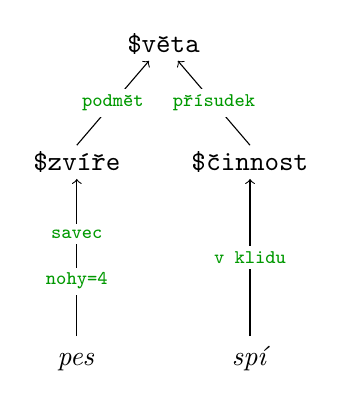
\begin{tikzpicture}[inner sep=2pt]
		\node (pes) at (0, 0) {\strut\emph{pes}};
		\node (spí) at (2.2, 0) {\strut\emph{spí}};
		\node (zvíře) at (0, 2.5) {\texttt{\$zvíře}};
		\node (činnost) at (2.2, 2.5) {\texttt{\$činnost}};
		\node (věta) at (1.1, 4) {\texttt{\$věta}};
		\draw[->] (pes.north) --
		node[pos=0.35, green!60!black,fill=white] {\scriptsize \texttt{nohy=4}}
		node[pos=0.65, green!60!black,fill=white] {\scriptsize \texttt{savec}}
		(zvíře.south);
		\draw[->] (spí.north) -- node[midway,green!60!black, fill=white] {\scriptsize \texttt{v klidu}} (činnost.south);
		\draw[->] (zvíře.north) -- node[midway, green!60!black,fill=white] {\scriptsize \texttt{podmět}} (věta);
		\draw[->] (činnost.north) -- node[midway, green!60!black, fill=white] {\scriptsize \texttt{přísudek}} (věta);
	\end{tikzpicture}
	\hspace{1cm}
	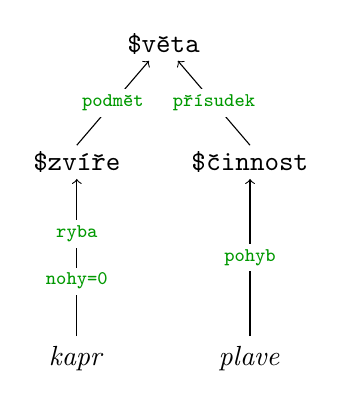
\begin{tikzpicture}[inner sep=2pt]
		\node (kapr) at (0, 0) {\strut\emph{kapr}};
		\node (plave) at (2.2, 0) {\strut\emph{plave}};
		\node (zvíře) at (0, 2.5) {\texttt{\$zvíře}};
		\node (činnost) at (2.2, 2.5) {\texttt{\$činnost}};
		\node (věta) at (1.1, 4) {\texttt{\$věta}};
		\draw[->] (kapr.north) --
		node[pos=0.35, green!60!black,fill=white] {\scriptsize \texttt{nohy=0}}
		node[pos=0.65, green!60!black,fill=white] {\scriptsize \texttt{ryba}}
		(zvíře.south);
		\draw[->] (plave.north) -- node[midway,green!60!black, fill=white] {\scriptsize \texttt{pohyb}} (činnost.south);
		\draw[->] (zvíře.north) -- node[midway, green!60!black,fill=white] {\scriptsize \texttt{podmět}} (věta);
		\draw[->] (činnost.north) -- node[midway, green!60!black, fill=white] {\scriptsize \texttt{přísudek}} (věta);
	\end{tikzpicture}
	\hspace{1cm}
	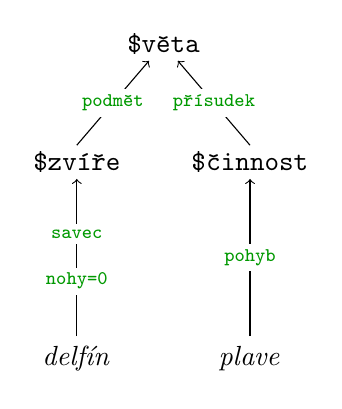
\begin{tikzpicture}[inner sep=2pt]
		\node (delfín) at (0, 0) {\strut\emph{delfín}};
		\node (plave) at (2.2, 0) {\strut\emph{plave}};
		\node (zvíře) at (0, 2.5) {\texttt{\$zvíře}};
		\node (činnost) at (2.2, 2.5) {\texttt{\$činnost}};
		\node (věta) at (1.1, 4) {\texttt{\$věta}};
		\draw[->] (delfín.north) --
		node[pos=0.35, green!60!black,fill=white] {\scriptsize \texttt{nohy=0}}
		node[pos=0.65, green!60!black,fill=white] {\scriptsize \texttt{savec}}
		(zvíře.south);
		\draw[->] (plave.north) -- node[midway,green!60!black, fill=white] {\scriptsize \texttt{pohyb}} (činnost.south);
		\draw[->] (zvíře.north) -- node[midway, green!60!black,fill=white] {\scriptsize \texttt{podmět}} (věta);
		\draw[->] (činnost.north) -- node[midway, green!60!black, fill=white] {\scriptsize \texttt{přísudek}} (věta);
	\end{tikzpicture}
	\caption{Derivační stromy s tagy}\label{fig:derivacni_stromy_tagy}
\end{figure}

Syntaxe SPGF je na Výpise~\ref{lst:spgf_syntax}, detaily implementace je možné
prozkoumat ve zdrojových kódech.
\begin{lstlisting}[
	% there are many more options of styling, see the official documentation, these are just the defaults I like
	frame=single, % make single-line frame around the verbatim
	framesep=2mm, % put some more spacing between the frame and text
	aboveskip=5mm, % put some more space above the box
	basicstyle={\linespread{1.0}\small\ttfamily}, % use typewriter (monospace) font
	caption={Syntaxe SPGF}, % set the caption text
	captionpos=b, % put the caption at the bottom (b) or top (t) or both (bt)
	label={lst:spgf_syntax}, % label to be referenced via \ref{}
	numbers=left, % line numbers on the left
	numberstyle={\scriptsize\ttfamily\color{black!60}}, % the style for line numbers
	escapeinside={<@}{@>} % between those sequences are command evaluated
]
grammar ::= rule+

rule ::= ('public' ' ')? ruleName '=' ruleBody ';'

ruleName ::= '$' unicodeAlphanumerical+

ruleBody ::= ruleAlternative ('|' ruleAlternative)*

ruleAlternative ::= element (' ' element)*

element ::= token | ruleRef | sequence

sequence ::= bracedSequence | optionalSequence

bracedSequence ::= '(' bareSequence ')'

optionalSequence ::= '[' bareSequence ']'

bareSequence ::= ruleAlternative ('|' ruleAlternative)*

token ::= (unicodeAlphanumerical | '.' | '-' | '_' | ':')+ 
          repeatOperator? tag*

repeatOperator ::=  '<' (('L' | 'G' | 'T') ':')? 
             (( digit+ '-' digit* ) | '*' | '+' | '?') '>'

ruleRef ::= '$' ruleName repeatOperator? tag*

tag ::= '{' [^}]+ '}'
\end{lstlisting}


\subsubsection{Parsovací strategie a opakování v SPGF}
Jak bylo zmíněno v sekci~\ref{subsubsec:spgf_def}, v gramatice je možné ke každému elementu,
s výjimkou speciálních pravidel \texttt{\$END}, \texttt{\$BEGIN}, \texttt{\$VOID} a \texttt{\$NULL},
přiřadit definici opakování.

Toto opakování udává, jaký je maximální a minimální počet bezprostředních opakování daného elementu během zpracování textu.
Například pokud má daný token specifikováno, že jeho minimální počet opakování je 2 a maximální 3,
tak v analyzovaném textu bude odpovídající slovo očekáváno dvakrát nebo třikrát po sobě.

Základní syntaxe je převzata ze standardu SRGS,
tedy dvě přirozená čísla oddělená pomlčkou (bez mezer) a ohraničené špičatými závorkami: \enquote{\texttt{<min-max>}}.
Pro pohodlnější zápis bylo definováno několik dalších alternativních
způsobů zápisu, viz Tabulka~\ref{tab:repeat_syntax}.
Pokud element žádné opakování nemá specifikované, implicitní hodnota je 1.

\begin{table}[ht!]
	\centering
	\def\width{14mm}
	\begin{tabular}{|l|p{\width}|p{\width}|l|}
		\hline
		\multirow{2}{*}{\textbf{Syntax}} & \multicolumn{2}{c|}{\textbf{Počet opakování}} & \multirow{2}{*}{\textbf{Poznámka}}                                               \\
		\cline{2-3}
		                                 & \textbf{min}                                  & \textbf{max}                       &                                             \\
		\hline
		\texttt{<m-n>}                   & $m$                                           & $n$                                & $m,n \in \mathbb{N}^{0} \ \wedge \ m\geq n$ \\
		\hline
		\texttt{<m->}                    & $m$                                           & $\infty$                           & v implementaci $\textbf{max} = 2^{32}-1$    \\
		\hline
		\texttt{<m>}                     & $m$                                           & $m$                                & ekvivalentní s \enquote{\texttt{<m-m>}}     \\
		\hline
		\texttt{<*>}                     & $0$                                           & $\infty$                           & ekvivalentní s \enquote{\texttt{<0->}}      \\
		\hline
		\texttt{<+>}                     & $1$                                           & $\infty$                           & ekvivalentní s \enquote{\texttt{<1->}}      \\
		\hline
		\texttt{<?>}                     & $0$                                           & $1$                                & ekvivalentní s \enquote{\texttt{<0-1>}}     \\
		\hline
	\end{tabular}
	\caption{Možné způsoby zápisu opakování v SPGF}\label{tab:repeat_syntax}
\end{table}

S opakovaným použitím stejného elementu je úzce spojena i strategie parsování.
Jedná se o způsob, jakým jsou řešené neurčité situace, kde je možné postupovat vícero způsoby.
Tyto situace mohou vznikat právě v místech opakování elementů, nebo tam, kde je k dispozici vícero aplikovatelných alternativ.

Konkrétní příklad jedné z možných nejednoznačných situací (přímo převzatý ze SRGS specifikace~\cite{srgs}) je v Tabulace~\ref{tab:ambiguity_example}.
Představuje situaci, kdy dvě alternativy mají různé tagy, ale stejné tokeny a tudíž není jasné, kterou z nich použít.
\begin{table}[ht!]
	\centering
	\begin{tabular}{|l|l|}
		\hline
		Expanze            & \texttt{t1 \{tag1\} | t1 \{tag2\} | t2} \\
		Vstupní řetězec    & \texttt{t1}                             \\
		Výstup (možnost 1) & \texttt{[{t1}, \{tag1\}]}               \\
		Výstup (možnost 2) & \texttt{[{t1}, \{tag2\}]}               \\
		\hline
	\end{tabular}
	\caption{Ukázka nejednoznačnosti SRGS}\label{tab:ambiguity_example}
\end{table}

V existující implementaci SRGS, se kterou byly prováděné první experimenty, byl implementován pouze takzvaný \enquote{hladový algoritmus}, běžněji označovaný pod anglickým názvem \emph{greedy matching}.
Pro potřeby sémantické analýzy textu v této práci bylo ovšem zjištěno, že pouze greedy algoritmus nebude zcela postačovat.
\todo{můžu takhle použít rovnou anglické názvy? přijdou mi lepší než české \enquote{hladový} \enquote{líný} nebo \enquote{důsledný}}

Příkladem takové situace by mohla být analýza textu
\begin{center}
	\emph{hnědý pes honí oranžovou malou veverku}
\end{center}
s cílem zjistit vlastnosti objektů (v tomto případě zvířat), zde konkrétně jejich barvy.
Pravidlo pro zachycení barvy zvířete by mohlo vypadat takto:
\begin{center}
	\texttt{public \$has\_color = \$color \$GARBAGE<*> \$animal;}
\end{center}
kde \texttt{\$color} a \texttt{\$animal} jsou reference na pravidla akceptující konkrétní slova pro barvy a zvířata.
Speciální pravidlo \texttt{\$GARBAGE} je zde definováno s operátorem opakování \enquote{\texttt{<*>}},
což lze chápat tak, že mezi samotnou barvou a zvířetem může být libovolný počet dalších slov, která nejsou podstatná.
Při zpracování textu pak ale dochází k problému, že greedy algoritmus vrátí derivační strom zakreslený na Obrázku~\ref{fig:parsing_tree_greedy}:
\begin{figure}[ht!]
	\centering
	\begin{tikzpicture}[inner sep=2pt]
		\def\dist{70pt}
		\foreach \w [count=\wi] in {hnědý, pes, honí, oranžovou, malou, veverku}
		\node (\w) at (\wi*\dist, 0) {\emph{\strut \w}};

		\def\dist{30pt}
		\node (r1) at ($(hnědý.north) + (0, \dist)$) {\strut\texttt{\$color}};
		\node (r2) at ($(pes.north) + (0, \dist)$) {\strut\texttt{\$GARBAGE}};
		\node (r3) at ($(honí.north) + (0, \dist)$) {\strut\texttt{\$GARBAGE}};
		\node (r4) at ($(oranžovou.north) + (0, \dist)$) {\strut\texttt{\$GARBAGE}};
		\node (r5) at ($(malou.north) + (0, \dist)$) {\strut\texttt{\$GARBAGE}};
		\node (r6) at ($(veverku.north) + (0, \dist)$) {\strut\texttt{\$animal}};

		\foreach \w [count=\wi] in {hnědý, pes, honí, oranžovou, malou, veverku}
		\draw[->] (\w.north) -- (r\wi.south);

		\node (color) at ($0.5*(r1.north west) + 0.5*(r6.north east) + (0, 1.5*\dist)$) {\strut \texttt{\$has\_color}};
		\foreach \n in {1,...,6}
		\draw[->] (r\n.north) -- (color);
	\end{tikzpicture}
	\caption{Derivační strom znázorňující problém s greedy algoritmem}\label{fig:parsing_tree_greedy}
\end{figure}

Jak je na derivačním stromu na Obrázku~\ref{fig:parsing_tree_greedy} vidět, následující sémantická analýza by došla pravděpodobně k závěru,
že v textu byla informace o hnědé veverce - což je chyba.
Zde speciální pravidlo \texttt{\$GARBAGE} s neomezeným počtem opakování v kombinaci s greedy algoritmem způsobilo,
že toto speciální pravidlo bylo \enquote{příliš agresivní} a aktivovalo se i v případech, kdy by již bylo možné použít následující element.

Z tohoto důvody byla do systému implementována druhá strategie, která se běžně označuje jako \emph{lazy matching}.
Zatímco greedy matching se v každém okamžiku snaží posunout parsování co nejdále, tato lazy strategie se naopak snaží použít element co nejméněkrát.

Také by se dalo říci, že pokud parsovací algoritmus narazí na element $e_{1}$ následovaný elementem $e_{2}$, pak:
\begin{itemize}
	\item greedy strategie se vždy nejdříve pokusí $e_{1}$ použít (opakovaně po sobě) a postoupí na $e_{2}$ až v moment, kdy
	      již není možné dále opakovat $e_{1}$,
	\item lazy strategie se vždy pokusí nejdříve postoupit na element $e_{2}$ a vrátí se k $e_{1}$ pro opakované použití až v moment,
	      kdy $e_{2}$ není možné použít
\end{itemize}

Implementace lazy strategie umožnila zachytit sémantiku, kterou by bylo obtížné získat pomocí greedy algoritmu.
Po několika dalších experimentech ovšem bylo zjištěno, že ani tato strategie nebude sama o sobě postačovat pro všechny potřeby sémantické analýzy.
Hlavním problémem s lazy strategií bylo to, že v textech, kde bylo více možných vyjádření stejného typu, byla detekována vždy jen ta nejkratší.

\newpage
Například předchozí úloha určování barev zvířat se vstupním textem
\begin{center}
	\emph{velký hnědý pes honí oranžovou malou veverku}
\end{center}
by mohla být zpracována SPGF pravidlem:
\begin{center}
	\texttt{public \$has\_color = \$GARBAGE<*> \$color \$GARBAGE<*> \$animal;}
\end{center}
V tomto případě bylo přidáno na začátek pravidla další \texttt{\$GARBAGE<*>}, které při použití lazy algoritmu způsobí,
že text nemusí začínat přímo barvou, ale je možné hledat barvy a zvířata až později v textu.
Derivační strom tohoto příkladu je zakreslen na Obrázku~\ref{fig:parsing_tree_lazy}.

\begin{figure}[ht!]
	\centering
	\begin{tikzpicture}[inner sep=2pt]
		\def\dist{55pt}
		\foreach \w [count=\wi] in {velký, hnědý, pes, honí, oranžovou, malou, veverku}
		\node (\w) at (\wi*\dist, 0) {\emph{\strut \w}};

		\def\dist{30pt}
		\node (r1) at ($(velký.north) + (0, \dist)$) {\strut\texttt{\$GARBAGE}};
		\node (r2) at ($(hnědý.north) + (0, \dist)$) {\strut\texttt{\$color}};
		\node (r3) at ($(pes.north) + (0, \dist)$) {\strut\texttt{\$animal}};

		\foreach \w [count=\wi] in {velký, hnědý, pes}
		\draw[->] (\w.north) -- (r\wi.south);

		\node (color) at ($0.5*(r1.north west) + 0.5*(r3.north east) + (0, 1.5*\dist)$) {\strut \texttt{\$has\_color}};
		\foreach \n in {1,...,3}
		\draw[->] (r\n.north) -- (color);

		\draw[thick, decorate, decoration={calligraphic brace, amplitude=5}]
		($(honí.north west) + (0, 0)$) -- ($(veverku.north east) + (0, 0)$)
		node[pos=0.5, above=4pt] {\scriptsize zbytek textu (není součástí derivačního stromu)};
	\end{tikzpicture}
	\caption{Derivační strom znázorňující problém s lazy algoritmem}\label{fig:parsing_tree_lazy}
\end{figure}
Z derivačního stromu na Obrázku~\ref{fig:parsing_tree_lazy} je možné usoudit, že následující sémantická analýza by pravděpodobně detekovala,
že v textu se nacházela informace o hnědém psovi - to je správně.
Nicméně je dále možné pozorovat, že v textu se vyskytovala také informace o oranžové veverce, kterou by systém nedokázal takto zachytit.

Z toho důvodu byl implementována ještě třetí strategie, která byla označena jako \enquote{\emph{thorough matching}}.
Myšlenka byla taková, že by bylo vhodné, aby algoritmus v místě nejednoznačnosti nemusel rozhodovat o tom,
který postup je nejlepší, ale aby místo toho uvažoval všechny možnosti.
Tento přístup se tedy od předchozích dvou liší v tom, že může vrátit pro jeden vstup více výstupů.

Základní koncept thorough strategie spočívá v tom, že v místě, kde by bylo možné postupovat vícero způsoby,
je řešení rozděleno do více paralelních větví (jedna pro každou možnost) a každá větev je dále zpracovávána nezávisle.
Tímto způsobem se rekurzivně vytváří strom možných řešení, jehož listy odpovídají finálním derivačním stromům.
Po ukončení všech těchto paralelních parsování jsou úspěšné výsledky vráceny jako seznam derivačních stromů.

Na výstupu tedy bude množina všech možných způsobů, jakým bylo možné derivační strom pro dané pravidlo a vstupní text sestavit.
To následně zaručí, že během zpracování textu nebyla opomenuta žádná sémantika
(za předpokladu, že jsou expertem správně sestavena parsovací pravidla).

Například pro předchozí úlohu určování barev zvířat se vstupním textem
\begin{center}
	\emph{velký hnědý pes honí oranžovou malou veverku}
\end{center}
a SPGF pravidlem:
\begin{center}
	\texttt{public \$has\_color = \$GARBAGE<*> \$color \$GARBAGE<*> \$animal;}
\end{center}
by výstupem byly 3 derivační stromy.
Dva z nich by byly shodné s výstupem greedy a lazy strategie (viz Obrázky~\ref{fig:parsing_tree_greedy} a~\ref{fig:parsing_tree_lazy}),
třetí (nový) derivační strom je na Obrázku~\ref{fig:parsing_tree_thorough}.

\begin{figure}[ht!]
	\centering
	\begin{tikzpicture}[inner sep=2pt]
		\def\dist{62pt}
		\foreach \w [count=\wi] in {velký, hnědý, pes, honí, oranžovou, malou, veverku}
		\node (\w) at (\wi*\dist, 0) {\emph{\strut \w}};

		\def\dist{30pt}
		\node (r1) at ($(velký.north) + (0, \dist)$) {\strut\texttt{\$GARBAGE}};
		\node (r2) at ($(hnědý.north) + (0, \dist)$) {\strut\texttt{\$GARBAGE}};
		\node (r3) at ($(pes.north) + (0, \dist)$) {\strut\texttt{\$GARBAGE}};
		\node (r4) at ($(honí.north) + (0, \dist)$) {\strut\texttt{\$GARBAGE}};
		\node (r5) at ($(oranžovou.north) + (0, \dist)$) {\strut\texttt{\$color}};
		\node (r6) at ($(malou.north) + (0, \dist)$) {\strut\texttt{\$GARBAGE}};
		\node (r7) at ($(veverku.north) + (0, \dist)$) {\strut\texttt{\$animal}};

		\foreach \w [count=\wi] in {velký, hnědý, pes, honí, oranžovou, malou, veverku}
		\draw[->] (\w.north) -- (r\wi.south);

		\node[ellipse] (color) at ($0.5*(r1.north west) + 0.5*(r7.north east) + (0, 1.5*\dist)$) {\strut \texttt{\$has\_color}};
		\foreach \n in {1,...,7}
		\draw[->] (r\n.north) -- (color);
	\end{tikzpicture}
	\caption{Derivační stromy z thorough algoritmu}\label{fig:parsing_tree_thorough}
\end{figure}

Celkově by tedy z tohoto výstupu bylo možné získat informace o tom, že v textu byla hnědá veverka, hnědý pes a oranžová veverka.
Dvě z těchto informací jsou správně, pouze informace o hnědé veverce je chybná, ta se v textu nevyskytla.

Jedná se o jednu z nevýhod thorough přístupu, že bude v textu hledat i takové informace, které z něj neplynou.
Tento problém byl vyřešen následnou filtrací získaných entit oproti referenčnímu popisu.
Detailní popis tohoto filtrování bude popsán v kapitole~\ref{subsubsec:algoritmus_zpracovani_stromu}.
% tak, že získané sémantické informace jsou porovnané s referenčním popisem obrázku a ty,
% které se v referenčním popise nevyskytují, jsou považované za falešně detekované a jsou z výstupu odstraněné
% (s výjimkou hodnot atributů, řešení chybných hodnot je popsáno v kapitole~\ref{subsec:hodnoceni}).

Tímto způsobem je pak v testovaném popisu pouze podmnožina referenčního popisu.
Jedná se o jednoduchý a efektivní způsob řešení falešně detekovaných sémantických informací.
Také ale bohužel představuje omezení v tom smyslu, že neumožňuje detekovat sémantiku, která se v textu skutečně nacházela,
ale nebyla zanesena do referenčního popisu - to klade očekávání na kvalitu referenčního popisu od experta.
Sestavení nějakého složitějšího algoritmu pro detekci falešně extrahované sémantiky představuje jedno z možných rozšíření do budoucna.

Další nevýhodou thorough strategie je její výpočetní náročnost.
Vzhledem k rekurzivnímu charakteru algoritmu a způsobu vytváření nových paralelních větví
se naskýtá riziko kombinatorické exploze počtu paralelních větví.
Během testování se však ukázalo, že pro moderní výpočetní techniku nepředstavují vstupy o velikosti desítek až stovek tokenů žádný problém.
Detailnější analýza výpočetní a paměťové náročnosti pro větší vstupy je nad rámec zadání a byla ponechána pro budoucí práce.

Posledním problémem, který bylo potřeba vyřešit v rámci parsovacích strategií, byl způsob, jakým strategie volit a přepínat.
V první verzi parseru se jednalo o globální přepínač, kdy bylo možné před samotným parsováním zvolit, jaká strategie má být použita.
Bylo ale zjištěno, že pro některé situace by bylo výhodné, aby bylo možné změnit výchozí strategii pro konkrétní pravidla nebo jejich části.

Například při zpracovávání číselných údajů je vhodná greedy strategie.
Je totiž potřeba, aby posloupnost sobě jdoucí slov, které reprezentující číselný údaj, byla brána jako jeden celek.

Jiný příklad pak může být již výše zmíněný začátek pravidla \texttt{\$GARBAGE<*>},
který libovolný počet prvních slov považovat za výplň a hledat tak význam až později v textu.
Pro tuto situaci je naopak greedy algoritmus zcela nevhodný, protože by celý text byl zpracován hned tímto počátkem.
Zde je vhodná lazy strategie, která ve své podstatě bude dávat přednost následujícím elementům
v pravidle a tento počátek bude používat až když zbytek pravidla selže.

Z těchto důvodů byla rozšířena syntaxe pro operátor definující opakování.
Před samotné hodnoty opakování (tedy hned za otevírací špičatou závorku \enquote{\texttt{<}}) je možné napsat
jedno z písmen \texttt{L}, \texttt{G}, \texttt{T} následované dvojtečkou a poté zbytek definice opakování.
Tato písmena odpovídají jednotlivým strategiím (lazy, greedy, thorough) a umožňují tak vynutit danou strategii pro dané pravidlo nebo jeho část.
Ve výsledku tak operátor opakování může vypadat například \enquote{\texttt{<G:1-3>}}, \enquote{\texttt{<L:*>}}, nebo \enquote{\texttt{<T:2->}}.

\subsection{Tvorba testovaného popisu}
Po implementaci systému pro zpracování přirozeného textu pomocí bezkontextových gramatik bylo potřeba získané derivační stromy nějakým způsobem
zpracovat a vytvořit z nich testovaný popis, který by bylo možné srovnat s referenčním popisem od experta.

Zpracování derivačních stromů obecně představuje konflikt mezi obtížností automatického zpracování a omezením na strukturu.
Striktně daná forma bude lépe zpracovatelná programově, ale může být obtížné zachytit všechny potřebné informace v dané struktuře.
Naopak více volná forma bude umožňovat snadnější zachycení různých typů informace, ale bude obtížnější sestavit algoritmus,
který by dokázal spolehlivě zpracovat předem neznámou strukturu.

Vzhledem k podobě testovaného a referenčního popisu, které byly popsané v kapitole~\ref{sec:navrh_architektura},
byl vytvořen algoritmus, který prochází získané derivační stromy a ukládá navštívené uzly s tagy do seznamu.
Z tohoto seznamu tagů pak určuje, jaká sémantická informace je v derivačním stromu obsažena.

Zde navržený přístup klade požadavek na způsob, jakým jsou sestavené SPGF gramatiky, protože předpokládá, že výstupní derivační stromy
budou mít takovou strukturu, aby při jejich procházení byly nalezené tagy v očekávaném pořadí.
Neklade tedy omezení přímo na strukturu samotných derivačních stromů, ale pouze na relativní rozmístění tagů uvnitř derivačního stromu.

\subsubsection{Algoritmus zpracování derivačních stromů}\label{subsubsec:algoritmus_zpracovani_stromu}
V první fázi algoritmus projde získaný derivační strom $T$ strategií depth-first-post-order (dfpo)~\cite{taocp1} a všechny navštívené tagy $t_{i}$ ukládá do seznamu.
Index $i$ značí index tagu odpovídající jeho pořadí při dfpo procházení stromu $T$.

Příklad takového stromu je na Obrázku~\ref{fig:tree_example}.
Zde je možné vidět, že ve skutečnosti tagy jsou realizované jako samostatné uzly, které následují vždy jako poslední (zleva doprava) uzel ke svému rodičovskému uzlu.
Při dfpo zpracování pak z tohoto stromu vznikne následující posloupnost tagů:
\begin{center}
	\texttt{[dog, part=obj, squirrel, part=subj, predicate=chasing, type=triplet]}
\end{center}

\begin{figure}[H]
	\centering
	\begin{tikzpicture}[inner sep=0pt,every node/.style={}]
		\def\dist{60pt}
		\foreach \w [count=\wi] in {velký, hnědý, pes, honí, oranžovou, malou, veverku}
		\node (\w) at (\wi*\dist, 0) {\emph{\strut \w}};

		\node (dog) at ($(pes.north) + (0, 50pt)$) {\strut\texttt{\$dog}};
		\node (g1) at ($(velký.north) + (0, 50pt)$) {\strut\texttt{\$GARBAGE}};
		\node (g2) at ($(hnědý.north) + (0, 50pt)$) {\strut\texttt{\$GARBAGE}};
		\node (obj1) at ($(dog.north) + (24pt, 50pt)$) {\strut\texttt{\$object}};
		\node (chasing) at ($(obj1.north) + (82pt, 50pt)$) {\strut\texttt{\$chasing}};
		\node (g3) at ($(oranžovou.north) + (0pt, 50pt)$) {\strut\texttt{\$GARBAGE}};
		\node (g4) at ($(malou.north) + (0, 50pt)$) {\strut\texttt{\$GARBAGE}};
		\node (squirrel) at ($(veverku.north) + (0, 50pt)$) {\strut\texttt{\$squirrel}};
		\node (obj2) at ($(squirrel.north) + (-60pt, 50pt)$) {\strut\texttt{\$object}};
		\node (triplet) at ($(chasing.north) + (0, 50pt)$) {\strut\texttt{\$triplet}};
		\node (output) at ($(triplet.north) + (-1, 50pt)$) {\strut\texttt{\$output}};

		\node[green!60!black, anchor=north west] (t1) at ($(dog.south east) + (0pt, -15pt)$) {\footnotesize\strut dog};
		\node[green!60!black, anchor=north west] (t2) at ($(obj1.south east) + (-26pt, -20pt)$) {\footnotesize\strut part=obj};
		\node[green!60!black, anchor=north west] (t3) at ($(squirrel.south east) + (-17.6pt, -15pt)$) {\footnotesize\strut squirrel};
		\node[green!60!black, anchor=north west] (t4) at ($(obj2.south east) + (30pt, -15pt)$) {\footnotesize\strut part=subj};
		\node[green!60!black, anchor=north west] (t5) at ($(chasing.south east) + (53pt, -19pt)$) {\footnotesize\strut predicate=chasing};
		\node[green!60!black, anchor=north west] (t6) at ($(triplet.south east) + (0pt, -15pt)$) {\footnotesize\strut type=triplet};
		\draw[-](t1) -- (dog);
		\draw[-](t2) -- (obj1);
		\draw[-](t3) -- (squirrel);
		\draw[-](t4) -- (obj2);
		\draw[-](t5) -- (chasing);
		\draw[-](t6) -- (triplet);

		\draw[-] (velký) to (g1);
		\draw[-] (hnědý) to (g2);
		\draw[-] (pes) to (dog);
		\draw[-] (honí) to (chasing);
		\draw[-] (oranžovou) to (g3);
		\draw[-] (malou) to (g4);
		\draw[-] (veverku) to (squirrel);
		\draw[-] (dog) to (obj1);
		\draw[-] (squirrel) to (obj2);
		\draw[-] (obj1) to (chasing);
		\draw[-] (obj2) to (chasing);
		\draw[-] (g3) to (chasing);
		\draw[-] (g4) to (chasing);
		\draw[-] (chasing) to (triplet);
		\draw[-] (triplet) to (output);
		\draw[-] (g1) to (output);
		\draw[-] (g2) to (output);

	\end{tikzpicture}
	\caption{Příklad derivačního stromu s tagy pro zpracování}\label{fig:tree_example}
\end{figure}

Získaný seznam tagů je postupně porovnáván s jednotlivými vzory, zda odpovídá nějaké předem definované sémantické informaci.
Rozlišované jsou tři typy informací, které odpovídají struktuře referenčního a testovaného popisu:
\begin{enumerate}
	\item \textbf{Objekty}: \\
	      Pro objekty stačí pouze identifikátor toho, že se jedná o objekt, a poté samotný název objektu.
	      Očekávaný seznam tagů tedy musí mít následující strukturu:
	      \begin{center}
		      $\bigl[ $ \emph{name},\ {\texttt{type=object}} $\bigr]$
	      \end{center}
	      kde \emph{name} je libovolný řetězec, který bude považován za název objektu.

	      Například při zpracování derivačního stromu, ze kterého bude získána posloupnost tagů
	      \texttt{[dog, type=object]},
	      bude extrahován objekt \enquote{\emph{dog}}, který bude poté přidán do testovaného popisu.
	\item \textbf{Atributy}: \\
	      Pro kompletní určení atributu je třeba identifikátor toho, že se jedná o atribut,
	      pak objekt, kterému je atribut přiřazen, následně název atributu a jeho hodnota.
	      Pro extrakci atributů byly definovány dvě různé struktury, kterých může seznam tagů nabývat:
	      \begin{center}
		      $\bigl[$ \emph{o\_name}, {\texttt{part=obj}}, \emph{a\_val}, \emph{a\_name},
					      {\texttt{part=attr}}, {\texttt{type=attribute}} $\bigr]$ \\
		      $\bigl[$ \emph{a\_val}, \emph{a\_name}, {\texttt{part=attr}}, \emph{o\_name},
					      {\texttt{part=obj}}, {\texttt{type=attribute}} $\bigr]$
	      \end{center}
	      kde \emph{o\_name}, \emph{a\_val} a \emph{a\_name} jsou libovolné řetězce, které budou považované za název objektu,
	      hodnotu atributu a název atributu.

	      Dvě různá očekávaná pořadí tagů vycházejí z toho, že v běžné mluvě lze specifikovat vlastnost objektu
	      před objektem (např.~\enquote{\emph{hnědý pes}}) i po něm (např.~\enquote{\emph{pes je hnědý}}).

	      Například při zpracování derivačního stromu, ze kterého budou získány tagy
	      \begin{center}
		      \texttt{[dog, part=obj, brown, color, part=attr, type=attribute]},
	      \end{center}
	      bude extrahován atribut \enquote{\emph{dog: color = brown}}, který bude poté přidán do testovaného popisu.
	\item \textbf{Vazby mezi objekty}:\\
	      Pro kompletní určení vazby mezi dvěma objekty je potřeba znát názvy obou objektů a název vazby mezi nimi.
	      Pro extrakci vazeb mezi objekty je očekáváno následující pořadí tagů:
	      \begin{center}
		      $\bigl[ $ \emph{from}, \texttt{part=obj}, \emph{to},
					      {\texttt{part=subj}}, \texttt{predicate=}\emph{pred}, {\texttt{type=triplet}} $\bigr]$
	      \end{center}
	      kde \emph{from}, \emph{to} a \emph{pred} jsou libovolné řetězce, které budou považované za název
	      zdrojového objektu, cílového objektu a název vazby.

	      Například při zpracování derivačního stromu, ze kterého budou získány tagy
	      \begin{center}
		      \texttt{[dog, part=obj, squirrel, part=subj, predicate=chasing, type=triplet]},
	      \end{center}
	      bude extrahován triplet \enquote{\emph{dog chasing squirrel}}, který bude poté přidán do testovaného popisu.
\end{enumerate}

Po extrakci objektů, atributů a tripletů jsou tyto získané sémantické informace profiltrovány,
za cílem odstranění falešně detekovaných entit.
Jak již bylo dříve zmíněno, filtrování probíhá tím způsobem, že pokud daný objekt, atribut,
nebo triplet nejsou v referenčním popisu, jsou ze seznamu odstraněné.
Výjimku tvoří atributy, kde je pouze chybná hodnota - tyto atributy jsou v seznamu ponechané a jsou uvažované v hodnocení,
jak bylo popsáno v kapitole~\ref{subsec:hodnoceni}.

\subsubsection{Číslování objektů}\label{subsubsec:cislovani_objektu}
Jeden z problémů, na který byl během implementace objeven, je absence číslování objektů.
Jak bylo popsáno v sekci~\ref{subsec:referencni_popis}, objekty mohou mít v rámci svého názvu číslování, kvůli jednoznačné rozlišitelnosti.
Nelze předpokládat, že by se tato číselná informace jakkoli vyskytovala v přirozeném popisu.
Naskýtá se tedy otázka, jak z přirozeného textu získat informaci o tom, o který objekt se konkrétně jedná
(za předpokladu, že daný objekt je v referenčním popise číslován).

Pro tento účel rozlišení číslovaných objektů byl sestaven doplňkový algoritmus,
který využívá unikátních vlastností objektů a jejich vazeb.
Hlavní myšlenka spočívá v tom, že pokud se názvy vícero objektů liší pouze číslováním,
pak je možné využít jejich atributy a vlastnosti k rozlišení, který objekt je který.

Například pokud ve scéně budou dva stromy \enquote{\texttt{strom \#1}} a \enquote{\texttt{strom \#2}} a právě jeden z nich
bude součástí tripletu \enquote{\texttt{veverka \to\ šplhá\_po \to\ strom \#1}}, pak lze například z textu:
\begin{center}
	\enquote{\emph{na obrázku vidím veverku, co šplhá po stromě}}
\end{center}
usoudit, že se jedná o \enquote{\texttt{strom \#1}}, protože \enquote{\texttt{strom \#2}} nemůže být součástí daného tripletu.
Je zde opět použit optimistický přístup, který předpokládá, že uživatel skutečně měl na mysli ten daný objekt (v tomto případě strom),
který se vyskytuje v detekovaném atributu či tripletu.

Na tomto principu byl tedy implementován algoritmus, který iterativně prochází extrahované informace z derivačních stromů
a postupně hledá, zda jsou v datech nějaké objekty, které by šly takto specifikovat.
Pokud je nějaký takový objekt nalezen, pak je mu přidáno příslušné číslování nejen v daném atributu nebo tripletu,
ale i ve všech ostatních extrahovaných datech, jelikož si vnitřní implementace udržuje informace o tom,
ze které části textu který kousek sémantiky pochází.

Dále se může stát, že specifikování jednoho objektu umožní následovné specifikování jiného objektu, protože dojde k eliminaci ostatních možností.
Tento iterativní algoritmus tedy prochází opakovaně všechna extrahovaná data až do chvíle,
než je celý průchod beze změny - v ten okamžik proces končí.

\subsection{Hodnotící algoritmus a ztrátová tabulka}
Po získání testovaného popisu je potřeba jej srovnat s referenčním popisem a ohodnotit míru jejich shody.
K tomuto účelu byl navržen a implementován hodnotící algoritmus, který byl detailně popsán v kapitole~\ref{subsec:hodnoceni}.

Vstupem jsou referenční popis získaný od experta, testovaný popis, jehož získání je popsáno v předchozích kapitolách a ztrátová tabulka,
která udává závažnost různých chyb.
Samotná ztrátová tabulka odpovídá svým formátem asociativnímu poli (též hash-tabulka nebo slovník), s předem danou strukturou.
Jelikož je SPGF systém citlivý na velikost písmen a interpunkční znaménka, jsou texty před vstupem normalizované
a zpracovávané větu po větě, výsledky pro jednotlivé věty jsou na konči sloučené.

Jak již bylo řečeno v kapitole~\ref{subsec:hodnoceni}, ztrátovou tabulku sestavuje expert, stejně jako referenční popis a SPGF gramatiky.
Z toho důvodu bylo nutné zvolit nějaký formát, který by byl čitelný člověkem a zároveň zpracovatelný strojem.
Zvolen byl opět formát \texttt{JSON}, který představuje dobrý kompromis mezi oběma faktory.
Ukázka ztrátové tabulky je na Výpisu~\ref{lst:loss_table_example}.

\begin{lstlisting}[
	% there are many more options of styling, see the official documentation, these are just the defaults I like
	frame=single, % make single-line frame around the verbatim
	framesep=2mm, % put some more spacing between the frame and text
	aboveskip=5mm, % put some more space above the box
	basicstyle={\linespread{0.9}\small\ttfamily}, % use typewriter (monospace) font
	caption={Ztrátová tabulka použitá při testování}, % set the caption text
	captionpos=b, % put the caption at the bottom (b) or top (t) or both (bt)
	label={lst:loss_table_example}, % label to be referenced via \ref{}
	numbers=left, % line numbers on the left
	numberstyle={\scriptsize\ttfamily\color{black!60}}, % the style for line numbers
	escapeinside={<@}{@>} % between those sequences are command evaluated
]
<@\textcolor[HTML]{FF1010}{\texttt{\{}}@>
<@\textcolor[HTML]{000000}{\texttt{\ \ }}@><@\textcolor[HTML]{255CFF}{\texttt{"missing\_objects"}}@><@\textcolor[HTML]{1041FF}{\texttt{:}}@><@\textcolor[HTML]{000000}{\texttt{\ }}@><@\textcolor[HTML]{DE6F10}{\texttt{3}}@><@\textcolor[HTML]{1041FF}{\texttt{,}}@>
<@\textcolor[HTML]{000000}{\texttt{\ \ }}@><@\textcolor[HTML]{255CFF}{\texttt{"missing\_attributes"}}@><@\textcolor[HTML]{1041FF}{\texttt{:}}@><@\textcolor[HTML]{000000}{\texttt{\ }}@><@\textcolor[HTML]{DE6F10}{\texttt{1}}@><@\textcolor[HTML]{1041FF}{\texttt{,}}@>
<@\textcolor[HTML]{000000}{\texttt{\ \ }}@><@\textcolor[HTML]{255CFF}{\texttt{"missing\_triplets"}}@><@\textcolor[HTML]{1041FF}{\texttt{:}}@><@\textcolor[HTML]{000000}{\texttt{\ }}@><@\textcolor[HTML]{DE6F10}{\texttt{2}}@><@\textcolor[HTML]{1041FF}{\texttt{,}}@>
<@\textcolor[HTML]{000000}{\texttt{\ \ }}@><@\textcolor[HTML]{255CFF}{\texttt{"numberless\_penalty"}}@><@\textcolor[HTML]{1041FF}{\texttt{:}}@><@\textcolor[HTML]{000000}{\texttt{\ }}@><@\textcolor[HTML]{DE6F10}{\texttt{0.5}}@><@\textcolor[HTML]{1041FF}{\texttt{,}}@>
<@\textcolor[HTML]{000000}{\texttt{\ \ }}@><@\textcolor[HTML]{255CFF}{\texttt{"wrong\_values"}}@><@\textcolor[HTML]{1041FF}{\texttt{:}}@><@\textcolor[HTML]{000000}{\texttt{\ }}@><@\textcolor[HTML]{DE6F10}{\texttt{2}}@><@\textcolor[HTML]{1041FF}{\texttt{,}}@>
<@\textcolor[HTML]{000000}{\texttt{\ \ }}@><@\textcolor[HTML]{255CFF}{\texttt{"missing\_objects\_override"}}@><@\textcolor[HTML]{1041FF}{\texttt{:}}@><@\textcolor[HTML]{000000}{\texttt{\ }}@><@\textcolor[HTML]{FF1010}{\texttt{[}}@>
<@\textcolor[HTML]{000000}{\texttt{\ \ \ \ }}@><@\textcolor[HTML]{FF1010}{\texttt{[}}@><@\textcolor[HTML]{418310}{\texttt{"person"}}@><@\textcolor[HTML]{1041FF}{\texttt{,}}@><@\textcolor[HTML]{000000}{\texttt{\ }}@><@\textcolor[HTML]{DE6F10}{\texttt{5}}@><@\textcolor[HTML]{FF1010}{\texttt{]}}@><@\textcolor[HTML]{1041FF}{\texttt{,}}@>
<@\textcolor[HTML]{000000}{\texttt{\ \ \ \ }}@><@\textcolor[HTML]{FF1010}{\texttt{[}}@><@\textcolor[HTML]{418310}{\texttt{"animal"}}@><@\textcolor[HTML]{1041FF}{\texttt{,}}@><@\textcolor[HTML]{000000}{\texttt{\ }}@><@\textcolor[HTML]{DE6F10}{\texttt{4}}@><@\textcolor[HTML]{FF1010}{\texttt{]}}@><@\textcolor[HTML]{1041FF}{\texttt{,}}@>
<@\textcolor[HTML]{000000}{\texttt{\ \ \ \ }}@><@\textcolor[HTML]{FF1010}{\texttt{[}}@><@\textcolor[HTML]{418310}{\texttt{"environment"}}@><@\textcolor[HTML]{1041FF}{\texttt{,}}@><@\textcolor[HTML]{000000}{\texttt{\ }}@><@\textcolor[HTML]{DE6F10}{\texttt{1}}@><@\textcolor[HTML]{FF1010}{\texttt{]}}@>
<@\textcolor[HTML]{000000}{\texttt{\ \ }}@><@\textcolor[HTML]{FF1010}{\texttt{]}}@><@\textcolor[HTML]{1041FF}{\texttt{,}}@>
<@\textcolor[HTML]{000000}{\texttt{\ \ }}@><@\textcolor[HTML]{255CFF}{\texttt{"missing\_attributes\_override"}}@><@\textcolor[HTML]{1041FF}{\texttt{:}}@><@\textcolor[HTML]{000000}{\texttt{\ }}@><@\textcolor[HTML]{FF1010}{\texttt{[}}@>
<@\textcolor[HTML]{000000}{\texttt{\ \ \ \ }}@><@\textcolor[HTML]{FF1010}{\texttt{[}}@><@\textcolor[HTML]{418310}{\texttt{"action"}}@><@\textcolor[HTML]{1041FF}{\texttt{,}}@><@\textcolor[HTML]{000000}{\texttt{\ }}@><@\textcolor[HTML]{DE6F10}{\texttt{1.5}}@><@\textcolor[HTML]{FF1010}{\texttt{]}}@><@\textcolor[HTML]{1041FF}{\texttt{,}}@>
<@\textcolor[HTML]{000000}{\texttt{\ \ \ \ }}@><@\textcolor[HTML]{FF1010}{\texttt{[}}@><@\textcolor[HTML]{418310}{\texttt{"state"}}@><@\textcolor[HTML]{1041FF}{\texttt{,}}@><@\textcolor[HTML]{000000}{\texttt{\ }}@><@\textcolor[HTML]{DE6F10}{\texttt{0.5}}@><@\textcolor[HTML]{FF1010}{\texttt{]}}@>
<@\textcolor[HTML]{000000}{\texttt{\ \ }}@><@\textcolor[HTML]{FF1010}{\texttt{]}}@><@\textcolor[HTML]{1041FF}{\texttt{,}}@>
<@\textcolor[HTML]{000000}{\texttt{\ \ }}@><@\textcolor[HTML]{255CFF}{\texttt{"missing\_triplets\_override"}}@><@\textcolor[HTML]{1041FF}{\texttt{:}}@><@\textcolor[HTML]{000000}{\texttt{\ }}@><@\textcolor[HTML]{FF1010}{\texttt{[}}@><@\textcolor[HTML]{FF1010}{\texttt{[}}@><@\textcolor[HTML]{418310}{\texttt{"falling\ into"}}@><@\textcolor[HTML]{1041FF}{\texttt{,}}@><@\textcolor[HTML]{000000}{\texttt{\ }}@><@\textcolor[HTML]{DE6F10}{\texttt{5}}@><@\textcolor[HTML]{FF1010}{\texttt{]}}@><@\textcolor[HTML]{FF1010}{\texttt{]}}@><@\textcolor[HTML]{1041FF}{\texttt{,}}@>
<@\textcolor[HTML]{000000}{\texttt{\ \ }}@><@\textcolor[HTML]{255CFF}{\texttt{"wrong\_values\_override"}}@><@\textcolor[HTML]{1041FF}{\texttt{:}}@><@\textcolor[HTML]{000000}{\texttt{\ }}@><@\textcolor[HTML]{FF1010}{\texttt{[}}@>
<@\textcolor[HTML]{000000}{\texttt{\ \ \ \ }}@><@\textcolor[HTML]{FF1010}{\texttt{\{}}@>
<@\textcolor[HTML]{000000}{\texttt{\ \ \ \ \ \ }}@><@\textcolor[HTML]{255CFF}{\texttt{"attribute"}}@><@\textcolor[HTML]{1041FF}{\texttt{:}}@><@\textcolor[HTML]{000000}{\texttt{\ }}@><@\textcolor[HTML]{418310}{\texttt{"color"}}@><@\textcolor[HTML]{1041FF}{\texttt{,}}@>
<@\textcolor[HTML]{000000}{\texttt{\ \ \ \ \ \ }}@><@\textcolor[HTML]{255CFF}{\texttt{"default"}}@><@\textcolor[HTML]{1041FF}{\texttt{:}}@><@\textcolor[HTML]{000000}{\texttt{\ }}@><@\textcolor[HTML]{DE6F10}{\texttt{0.5}}@><@\textcolor[HTML]{1041FF}{\texttt{,}}@>
<@\textcolor[HTML]{000000}{\texttt{\ \ \ \ \ \ }}@><@\textcolor[HTML]{255CFF}{\texttt{"overrides"}}@><@\textcolor[HTML]{1041FF}{\texttt{:}}@><@\textcolor[HTML]{000000}{\texttt{\ }}@><@\textcolor[HTML]{FF1010}{\texttt{[}}@>
<@\textcolor[HTML]{000000}{\texttt{\ \ \ \ \ \ \ \ }}@><@\textcolor[HTML]{FF1010}{\texttt{[}}@><@\textcolor[HTML]{FF1010}{\texttt{[}}@><@\textcolor[HTML]{418310}{\texttt{"white"}}@><@\textcolor[HTML]{1041FF}{\texttt{,}}@><@\textcolor[HTML]{000000}{\texttt{\ }}@><@\textcolor[HTML]{418310}{\texttt{"yellow"}}@><@\textcolor[HTML]{1041FF}{\texttt{,}}@><@\textcolor[HTML]{000000}{\texttt{\ }}@><@\textcolor[HTML]{418310}{\texttt{"pink"}}@><@\textcolor[HTML]{FF1010}{\texttt{]}}@><@\textcolor[HTML]{1041FF}{\texttt{,}}@><@\textcolor[HTML]{000000}{\texttt{\ }}@><@\textcolor[HTML]{DE6F10}{\texttt{0.3}}@><@\textcolor[HTML]{FF1010}{\texttt{]}}@><@\textcolor[HTML]{1041FF}{\texttt{,}}@>
<@\textcolor[HTML]{000000}{\texttt{\ \ \ \ \ \ \ \ }}@><@\textcolor[HTML]{FF1010}{\texttt{[}}@><@\textcolor[HTML]{FF1010}{\texttt{[}}@><@\textcolor[HTML]{418310}{\texttt{"red"}}@><@\textcolor[HTML]{1041FF}{\texttt{,}}@><@\textcolor[HTML]{000000}{\texttt{\ }}@><@\textcolor[HTML]{418310}{\texttt{"blue"}}@><@\textcolor[HTML]{1041FF}{\texttt{,}}@><@\textcolor[HTML]{000000}{\texttt{\ }}@><@\textcolor[HTML]{418310}{\texttt{"green"}}@><@\textcolor[HTML]{1041FF}{\texttt{,}}@><@\textcolor[HTML]{000000}{\texttt{\ }}@><@\textcolor[HTML]{418310}{\texttt{"yellow"}}@><@\textcolor[HTML]{FF1010}{\texttt{]}}@><@\textcolor[HTML]{1041FF}{\texttt{,}}@><@\textcolor[HTML]{000000}{\texttt{\ }}@><@\textcolor[HTML]{DE6F10}{\texttt{0.8}}@><@\textcolor[HTML]{FF1010}{\texttt{]}}@>
<@\textcolor[HTML]{000000}{\texttt{\ \ \ \ \ \ }}@><@\textcolor[HTML]{FF1010}{\texttt{]}}@>
<@\textcolor[HTML]{000000}{\texttt{\ \ \ \ }}@><@\textcolor[HTML]{FF1010}{\texttt{\}}}@><@\textcolor[HTML]{1041FF}{\texttt{,}}@>
<@\textcolor[HTML]{000000}{\texttt{\ \ \ \ }}@><@\textcolor[HTML]{FF1010}{\texttt{\{}}@>
<@\textcolor[HTML]{000000}{\texttt{\ \ \ \ \ \ }}@><@\textcolor[HTML]{255CFF}{\texttt{"attribute"}}@><@\textcolor[HTML]{1041FF}{\texttt{:}}@><@\textcolor[HTML]{000000}{\texttt{\ }}@><@\textcolor[HTML]{418310}{\texttt{"action"}}@><@\textcolor[HTML]{1041FF}{\texttt{,}}@>
<@\textcolor[HTML]{000000}{\texttt{\ \ \ \ \ \ }}@><@\textcolor[HTML]{255CFF}{\texttt{"default"}}@><@\textcolor[HTML]{1041FF}{\texttt{:}}@><@\textcolor[HTML]{000000}{\texttt{\ }}@><@\textcolor[HTML]{DE6F10}{\texttt{1.5}}@><@\textcolor[HTML]{1041FF}{\texttt{,}}@>
<@\textcolor[HTML]{000000}{\texttt{\ \ \ \ \ \ }}@><@\textcolor[HTML]{255CFF}{\texttt{"overrides"}}@><@\textcolor[HTML]{1041FF}{\texttt{:}}@><@\textcolor[HTML]{000000}{\texttt{\ }}@><@\textcolor[HTML]{FF1010}{\texttt{[}}@>
<@\textcolor[HTML]{000000}{\texttt{\ \ \ \ \ \ \ \ }}@><@\textcolor[HTML]{FF1010}{\texttt{[}}@><@\textcolor[HTML]{FF1010}{\texttt{[}}@><@\textcolor[HTML]{418310}{\texttt{"sitting"}}@><@\textcolor[HTML]{1041FF}{\texttt{,}}@><@\textcolor[HTML]{000000}{\texttt{\ }}@><@\textcolor[HTML]{418310}{\texttt{"reading"}}@><@\textcolor[HTML]{FF1010}{\texttt{]}}@><@\textcolor[HTML]{1041FF}{\texttt{,}}@><@\textcolor[HTML]{000000}{\texttt{\ }}@><@\textcolor[HTML]{DE6F10}{\texttt{0.8}}@><@\textcolor[HTML]{FF1010}{\texttt{]}}@><@\textcolor[HTML]{1041FF}{\texttt{,}}@>
<@\textcolor[HTML]{000000}{\texttt{\ \ \ \ \ \ \ \ }}@><@\textcolor[HTML]{FF1010}{\texttt{[}}@><@\textcolor[HTML]{FF1010}{\texttt{[}}@><@\textcolor[HTML]{418310}{\texttt{"fishing"}}@><@\textcolor[HTML]{1041FF}{\texttt{,}}@><@\textcolor[HTML]{000000}{\texttt{\ }}@><@\textcolor[HTML]{418310}{\texttt{"sitting"}}@><@\textcolor[HTML]{FF1010}{\texttt{]}}@><@\textcolor[HTML]{1041FF}{\texttt{,}}@><@\textcolor[HTML]{000000}{\texttt{\ }}@><@\textcolor[HTML]{DE6F10}{\texttt{0.7}}@><@\textcolor[HTML]{FF1010}{\texttt{]}}@>
<@\textcolor[HTML]{000000}{\texttt{\ \ \ \ \ \ }}@><@\textcolor[HTML]{FF1010}{\texttt{]}}@>
<@\textcolor[HTML]{000000}{\texttt{\ \ \ \ }}@><@\textcolor[HTML]{FF1010}{\texttt{\}}}@>
<@\textcolor[HTML]{000000}{\texttt{\ \ }}@><@\textcolor[HTML]{FF1010}{\texttt{]}}@>
<@\textcolor[HTML]{FF1010}{\texttt{\}}}@>

\end{lstlisting}


Význam jednotlivých položek byl detailně popsán v sekci~\ref{subsec:hodnoceni}, proto zde bude pouze stručně shrnuto,
který klíč odpovídá jakému významu:
\begin{itemize}
	\item \texttt{missing\_objects} \to\ výchozí ztráta pro chybějící objekty
	\item \texttt{missing\_attributes} \to\ výchozí ztráta pro chybějící atributy
	\item \texttt{missing\_triplets} \to\ výchozí ztráta pro chybějící triplety (vazby)
	\item \texttt{numberless\_penalty} \to\ ztráta pro informace obsahující objekty s chybějícím číslováním (viz sekce~\ref{subsubsec:cislovani_objektu})
	\item \texttt{wrong\_value} \to\ výchozí ztráta pro atributy s chybnou hodnotou
	\item \texttt{missing\_objects\_override} \to\ seznam konkrétních ztrát pro chybějící objekty s daným tagem
	\item \texttt{missing\_attributes\_override} \to\ seznam konkrétních ztrát pro chybějící atributy (podle názvu atributu)
	\item \texttt{missing\_triplets\_override} \to\ seznam konkrétních ztrát pro chybějící triplety (podle názvu vazby)
	\item \texttt{wrong\_values\_override} \to\ seznam konkrétních ztrát pro daný atribut a případně i pro záměnu konkrétních hodnot
\end{itemize}

Finálním výstupem hodnotícího algoritmu je množina označených číselných hodnot, získaných akumulací ztrát pro různé druhy chyb.
Přirozenou datovou strukturou, která by odpovídala tomuto formátu, by bylo asociativní pole (někdy také označované jako hash-tabulka, nebo slovník).

Příkladem takového výstupu může být Výpis~\ref{lst:output_example}:
\begin{lstlisting}[
	% there are many more options of styling, see the official documentation, these are just the defaults I like
	frame=single, % make single-line frame around the verbatim
	framesep=2mm, % put some more spacing between the frame and text
	aboveskip=5mm, % put some more space above the box
	basicstyle={\linespread{0.9}\small\ttfamily}, % use typewriter (monospace) font
	caption={Ukázka výpisu hodnocení (zkráceno)}, % set the caption text
	captionpos=b, % put the caption at the bottom (b) or top (t) or both (bt)
	label={lst:output_example}, % label to be referenced via \ref{}
	numbers=left, % line numbers on the left
	numberstyle={\scriptsize\ttfamily\color{black!60}}, % the style for line numbers
	% escapeinside={<@}{@>} % between those sequences are command evaluated
]
missing_objects: 125.5,
missing_attributes: 79.5,
missing_triplets: 164.0,
wrong_values: 0.0,
grouped_missing_objects: {
    "group": 21.0,
    "item": 24.0,
    "person": 5.5,
    "animal": 52.0,
    "clothing": 24.0,
    ...
},
grouped_missing_attributes: {
    "hairstyle": 1.0,
    "pattern": 1.0,
    "action": 5.0,
    "color": 61.0,
    ...
},
grouped_missing_triplets: {
    "reading": 0.0,
    "climbing": 2.0,
    "throwing": 2.0,
    "playing with": 6.0,
    "chasing": 2.0,
    "swimming in": 2.0,
    "following": 10.0,
    ...
},
grouped_wrong_values: {
    "state": 0.0,
    "facial expression": 0.0,
    "pattern": 0.0,
    "color": 0.0,
    ...
},
\end{lstlisting}

